\documentclass[a4paper]{article}

\usepackage[intlimits]{amsmath}
\usepackage{mathrsfs}
\usepackage{amsthm}
\usepackage{amssymb}
\usepackage{cancel}
\usepackage{graphicx}
\usepackage{color}
\usepackage{natbib}
\usepackage{hyperref}
\usepackage{listings}
\usepackage{parskip}
\usepackage[margin=1.3in]{geometry}
\usepackage[nottoc,numbib]{tocbibind}
\usepackage{abstract}
\usepackage{multicol}
\usepackage{float}

\citestyle{apalike}
\bibliographystyle{apalike}

\providecommand{\e}[1]{\times10^{#1}}
\providecommand{\units}[1]{\;\mathrm{#1}}
\providecommand{\data}[2]{$#1\units{#2}$}
\providecommand{\diff}[2]{\frac{\partial #1}{\partial #2}}
\providecommand{\ddiff}[2]{\frac{\partial^2 #1}{\partial #2^2}}
\providecommand{\tdiff}[2]{\frac{\mathrm{d} #1}{\mathrm{d} #2}}
\providecommand{\infint}[2]{\int\limits_{-\infty}^{\infty}{#1}\;\mathrm{d}#2}
\providecommand{\dd}{\;\mathrm{d}}
\providecommand{\MAA}{\text{\AA}}
\providecommand{\abs}[1]{\left| #1 \right|} % for absolute value
\providecommand{\avg}[1]{\left< #1 \right>} % for average
\providecommand{\grad}[1]{\gv{\nabla} #1} % for gradient
\let\divsymb=\div
\renewcommand{\div}[1]{\gv{\nabla} \cdot #1} % for divergence
\providecommand{\curl}[1]{\gv{\nabla} \times #1} % for curl
\providecommand{\MAA}{\text{\AA}}
\providecommand{\figwidth}{.45\columnwidth}
\newcommand\numberthis{\addtocounter{equation}{1}\tag{\theequation}}
\numberwithin{equation}{section}

\setlength\columnsep{14pt}

\renewcommand{\bibname}{References}

\title{Characterising Interstellar Dust with Herschel-SPIRE\thanks{{\it Herschel} is an ESA space observatory with science instruments provided by European-led Principal Investigator consortia and with important participation from NASA.}: \\ \large{Evaluation of a super-resolution technique for high signal to noise SPIRE maps}}
\author{Tom Badran}

\date{September 2014 to May 2015}

\begin{document}

\maketitle
\begin{abstract}
%!TEX root = spire-project.tex
The photometers contained within the Herschel SPIRE instrument have an angular resolution limited only by diffraction, where the $500\units{\mu m}$ photometer is limited to an angular resolution of approximately 35''. Here I present an investigation into the use of a super-resolution technique (HiRes) first implemented for IRAS. A set of possible methodologies for quantifying the performance of HiRes is presented, and a method where measuring RMS pixel differences for a synthetic observation is identified as a suitable way to quantify the HiRes improvement of an unmodified observation. Also established is a possible threshold of 99th percentile peak SNR of \textgreater30 where HiRes can be automatically applied to an observation as part of the work of the SPIRE post operations team.

\end{abstract}

\tableofcontents

\listoffigures
%\listoftables
\break
\begin{multicols}{2}
\raggedcolumns

\section{Introduction}
\subsection{Aims and Objectives}

The primary aim of the project is to assist the SPIRE Post-Operations Team in the evaluation of the HIRES routine to enhance angular resolution of SPIRE maps. A procedure for evaluating the effectiveness of HiRes on an observation and set of criteria for establishing whether to use HiRes on an observation should be used needs to be established before September 2015.

This will require analyzing the output of HiRes and establishing a metric for determining the level of improvement (if any) provided on an existing observation.

The method proposed for this is to generate simulated observational data from a higher resolution source, and then use this as a basis of comparison for testing the effectiveness of HiRes, focusing on how the signal to noise of an observation effects the fidelity of HiRes images.

It is proposed that examining the power spectra of both the simulated observations and the output of HiRes, and comparing these to the power spectra of the higher resolution source material may reveal useful information. Additionally the extra information returned by the HiRes routine may hold details about effectiveness. Difference maps of the images produced may also hold other information, and most importantly reveal if any additional artifacts are created.


%!TEX root = spire-project.tex
\subsection{Dust Emission}

To measure the size and mass of optically thick molecular clouds, we can not simply look at the starlight passing through them, we must instead look at the emission from the dust \citep{hildebrand1983determination}. For very cool clouds (\textless 20K) the emission from the dust grains is in the far-infrared and submillimetre wavelengths.

Observations at these wavelengths are generally not possible from ground based telescopes due to atmospheric absorption \citep{houghton2002physics} so instead they are observed from space based observing platforms such as IRAS, Spitzer and Herschel.

\subsection{Blackbody Radiation}

All bodies at finite temperature emit EM radiation; a body in thermal equilibrium with its environment will emit according to a blackbody spectrum. While classical descriptions explained a portion of this radiation, it was not until the early 1900's that Max Planck described this emission fully \citep{planck1914theory}. Planck developed his model using quantum theory, first developing his theory as an improvement to the Wein approximation \citep{wien1897} using empirically measured constants, and later developing a physical derivation by considering the energies of photons inside a box at thermal equilibrium. Planck derived an expression for the spectral radiance of a body, which can be expressed in terms of different spectral variables, e.g. in terms of frequency in equation \ref{bbf} and wavelength, as in equation \ref{bbw}.

\begin{figure}[H]
    \centering
    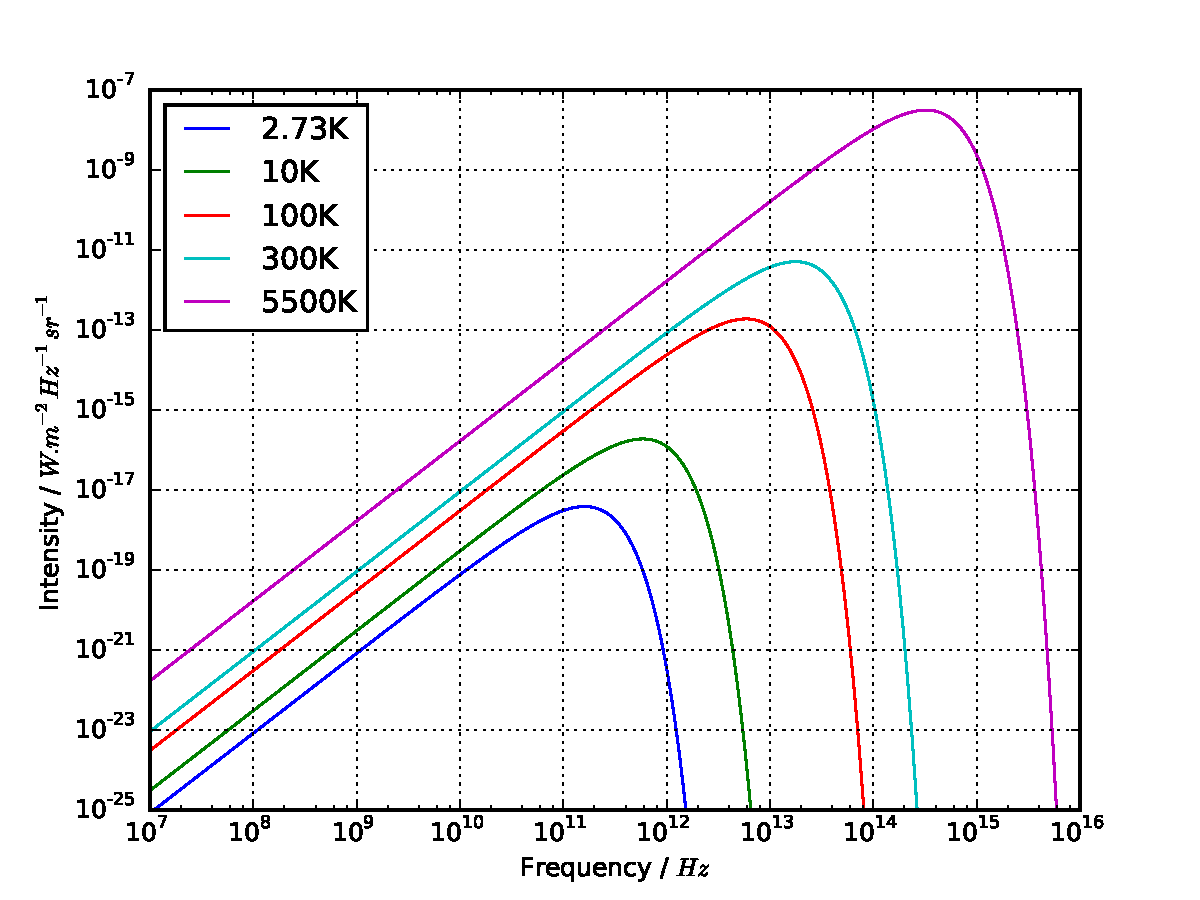
\includegraphics[width=\linewidth]{figures/bb10k.pdf}
    \caption{Blackbody spectrum for bodies at various temperatures}
    \label{bb10k}
\end{figure}

\begin{equation}
    \label{bbf}
    B_\nu(\nu,T) = \frac{2h\nu^3}{c^2}\left( e^{\frac{h\nu}{k_bT}} - 1\right)^{-1}
\end{equation}

\begin{equation}
    \label{bbw}
    B_\lambda(\lambda,T) = \frac{2hc^2}{\lambda^5}\left( e^{\frac{hc}{\lambda k_bT}} - 1\right)^{-1}
\end{equation}

For a blackbody at $10\units{K}$, i.e. typical cold cosmic dust, the spectral radiance will look as shown in Figure \ref{bb10k}, with a peak at approximately $290\units{\mu m}$.

\subsection{How to observe}

\subsubsection{Angular Resolution}

The resolution of any optical system is limited by two factors, aberration and diffraction. Aberrations can be considered to be caused by any defect in the optical system, so can be overcome simply by the use of better construction techniques and use of higher quality materials. In well constructed optical devices, such as modern telescopes, the resolution of any image produced is then limited only by the diffraction of the optical system.

Due to the wave like nature of light, any light passing through an aperture will undergo diffraction. Light from a point source such as a star, passing through a circular aperture will appear in the focal plane as a circular image with a series of rings surrounding it as shown in Figure \ref{airy}. Lord Rayleigh defined a criterion for defining when two objects are resolvable from each other as when the diffraction maximum of one of the objects coincides with the first minimum of the second object \citep{rayleigh1880v}.

\begin{figure}[H]
    \centering
    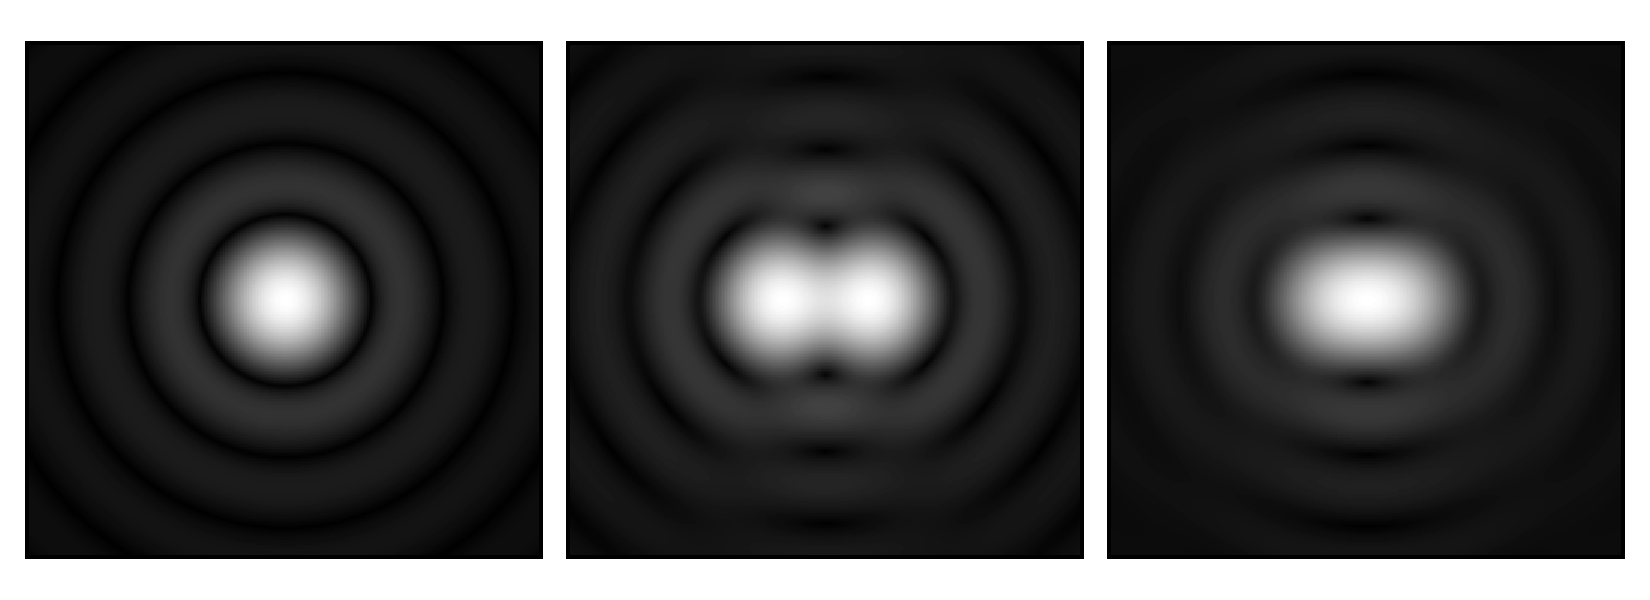
\includegraphics[width=\linewidth]{figures/airy.pdf}
    \caption[Point spread functions]{Point spread functions, from left to right, the Airy disk for a point source, two point sources at the Rayleigh criterion, and two indistinguishable point sources}
    \label{airy}
\end{figure}

Equation \ref{angularres} gives the angular resolution on the sky, as determined by the aperture diameter of the telescope and the wavelength of light. The quality of the images then will increase as $\theta$ decreases, i.e. the angular size of resolvable objects becomes smaller. Clearly as equation \ref{angularres} shows, the resolution then worsens as the wavelength increases, and increases as the diameter of the telescope aperture increases. The telescope beam itself will have a FWHM of approximately $\lambda/D$. As the observation wavelengths are largely determined by the type of objects being observed, the only practical way to improve the the angular resolution is then to increase the telescope aperture size. This of course has the downside of being very expensive, and in the case of space telescopes impractical due to limitations of the launch systems. NASA has a report claiming that the cost of a space telescope is related to the diameter by equation \ref{nasacost} \citep{stahl2011update}.

\begin{equation}
    \theta = 1.22 \frac{\lambda}D
    \label{angularres}
\end{equation}

\begin{equation}
    \text{Cost} \propto D^{1.4}
    \label{nasacost}
\end{equation}

It is therefore very advantageous to find any mechanism to help increase the angular resolution of the observations without incurring additional costs in the telescope construction, or cost of the missions required to launch space telescopes.

\subsubsection{IR detection using Bolometers}

Detection of submillimetre radiation is not possible with CCD technology as is used for imaging in optical and some near optical infra-red detectors \citep{janesick2001scientific}. CCDs work in principle by having electrons released by photo-excitation, and collected into a potential well before measurement. While CCDs have excellent quantum efficiencies (the ratio of incident photons converted to electron-hole pairs) in and around optical wavelength bands, their response falls off around $1\units{\mu m}$ because the photons are no longer energetic enough to produce electron-hole pairs.

Equation \ref{photonenergy} shows that the energy of a photon is inversely proportional to the wavelength. Clearly optical and near infra red photons will have a higher energy than sub millimeter photons, so much so that there is no material that can act as a CCD for submillimetre photons; instead a different method of detection is required.

\begin{equation}
    E = \frac{hc}{\lambda}
    \label{photonenergy}
\end{equation}

Instead of using CCD type devices, one can use bolometers to detect the photons. The principal mechanism of bolometer operation is different to CCDs in that it does not rely on the excitation of electrons (Figure \ref{bolometer}). Instead, as the photons do not have high enough energy, they simply cause atoms in some absorbing material to become thermally excited. This action then changes the resistivity of the material which is something that can be measured.

\begin{figure}[H]
    \centering
    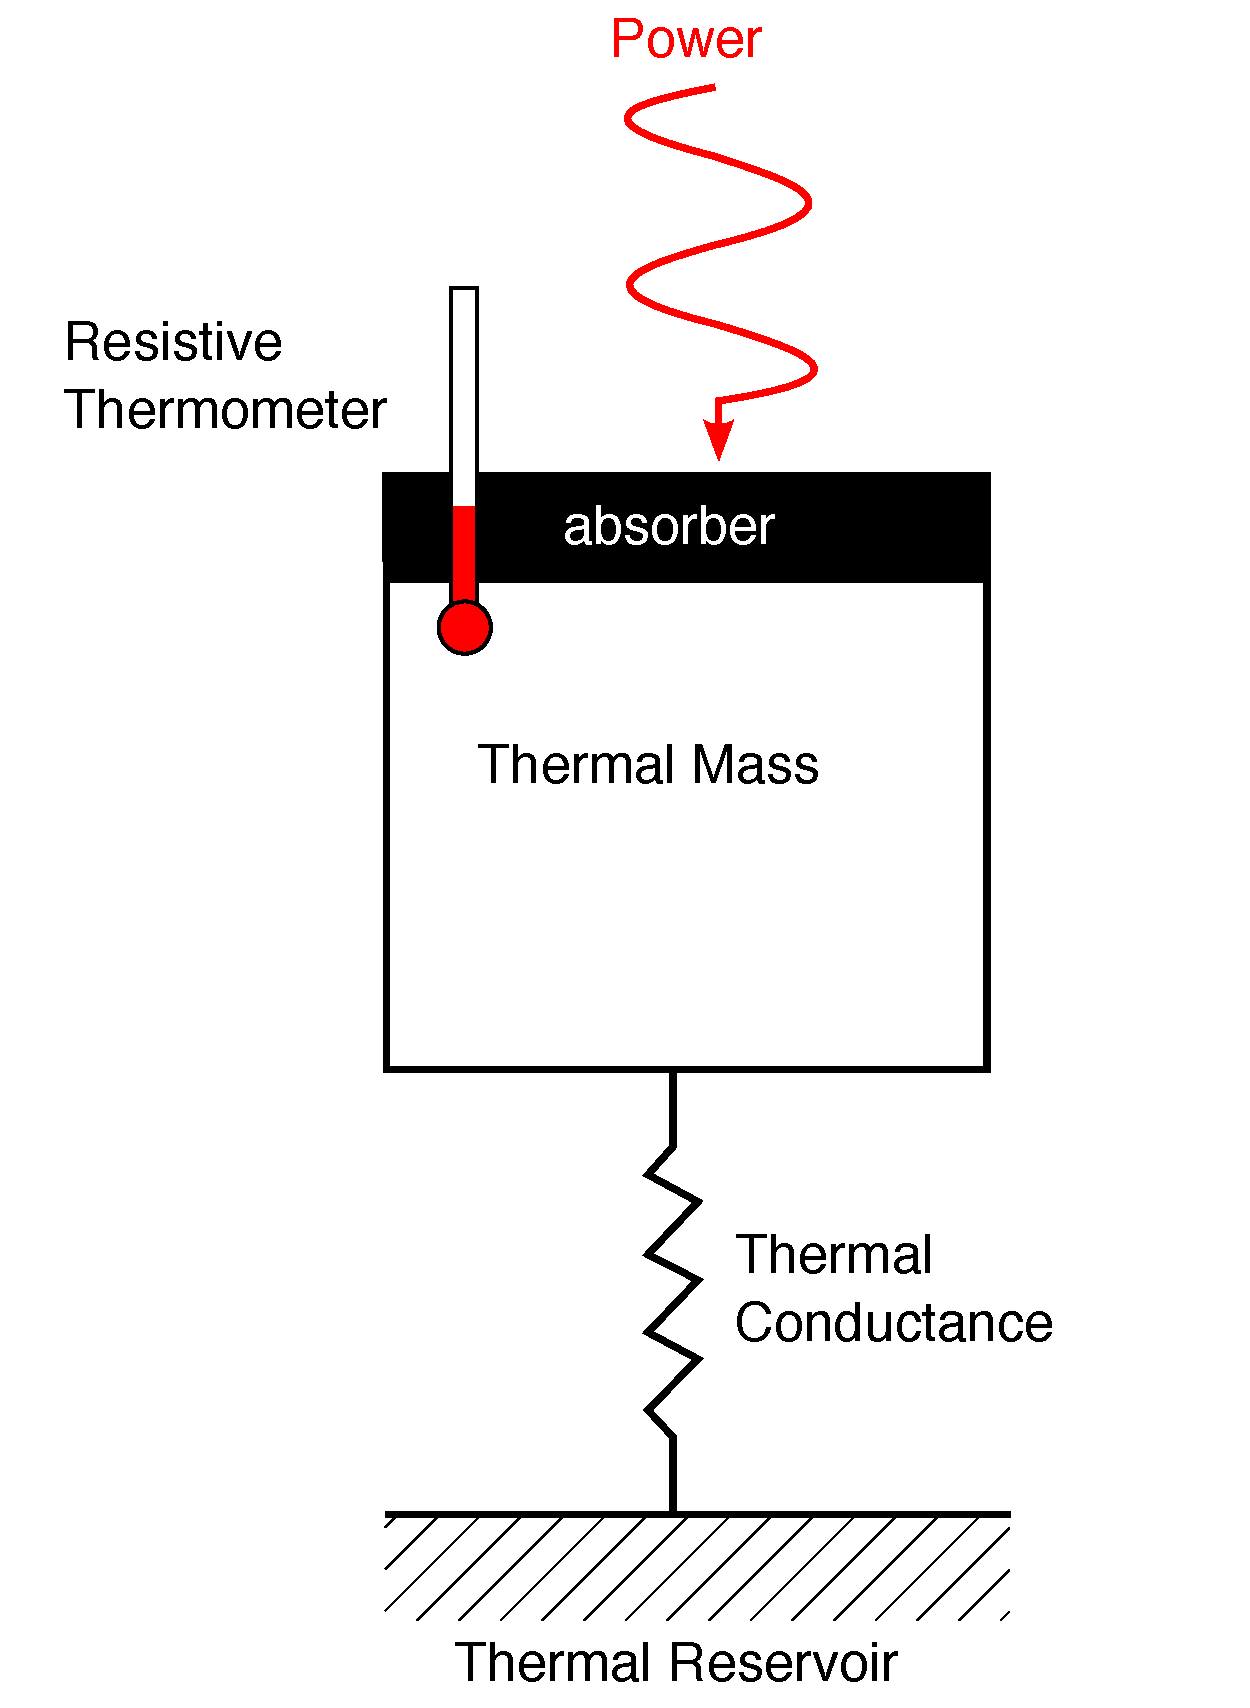
\includegraphics[width=0.8\linewidth]{figures/bolometer.pdf}
    \caption[Conceptual operation of a Bolometer]{Conceptual operation of a Bolometer \citep{bolometerSchematic}}
    \label{bolometer}
\end{figure}

While thermal noise is an issue for CCDs, it is a much bigger problem with bolometers. In order to get accurate readings, the whole device needs to be kept very cold, down to a below $100\units{mK}$ in some cases, and the time response for the thermal energy to flow into the thermal reservoir needs to be carefully calibrated and well understood for any particular device. Any thermal noise can easily drown out any useful signal measurable.

\subsection{Sampling Theory}

Information theory was developed in 1948 by Claude Shannon \citep{shannon2001mathematical} in order to find the fundamental limits of signal processing. The theory describes how much information is needed to convey some message through a communications channel, but the mathematics apply to how information can be sampled from some measurable phenomenon.

The theory was expanded into the field of digital signal processing, where it was established that the sampling rate required to obtain all the information from a continuous time signal is twice the highest frequency in the signal. So for instance to capture the signal from a pure sine wave at $1\units{Hz}$, measurements would need to be taken at a frequency of $2\units{Hz}$.

\subsection{Herschel Space Observatory}

The Herschel space observatory was launched by the ESA on the 14th of May, 2009, observing in the far infrared and submillimetre range of the EM spectrum, using a Cassegrain design with a $3.5\units{m}$ primary mirror. Herschel has two direct detection instruments, i.e. they measure the intensity of the incident radiation, PACS and SPIRE, and a high-resolution spectrometer, HIFI. The PACS imaging photometer observes at $70\units{\mu m}$, $100\units{\mu m}$ and $160\units{\mu m}$ and the SPIRE imaging photometer observes at 3 bands, $250\units{\mu m}$, $350\units{\mu m}$ and $500\units{\mu m}$ \citep{pilbratt2010herschel}. Note that combining the data from both PACS and SPIRE allows us to fit six data points to the blackbody spectrum. PACS and SPIRE also have spectrometers, although spectrographic data is not used in this project so these will not be discussed further.

\subsubsection{Herschel SPIRE}

\begin{figure}[H]
    \centering
    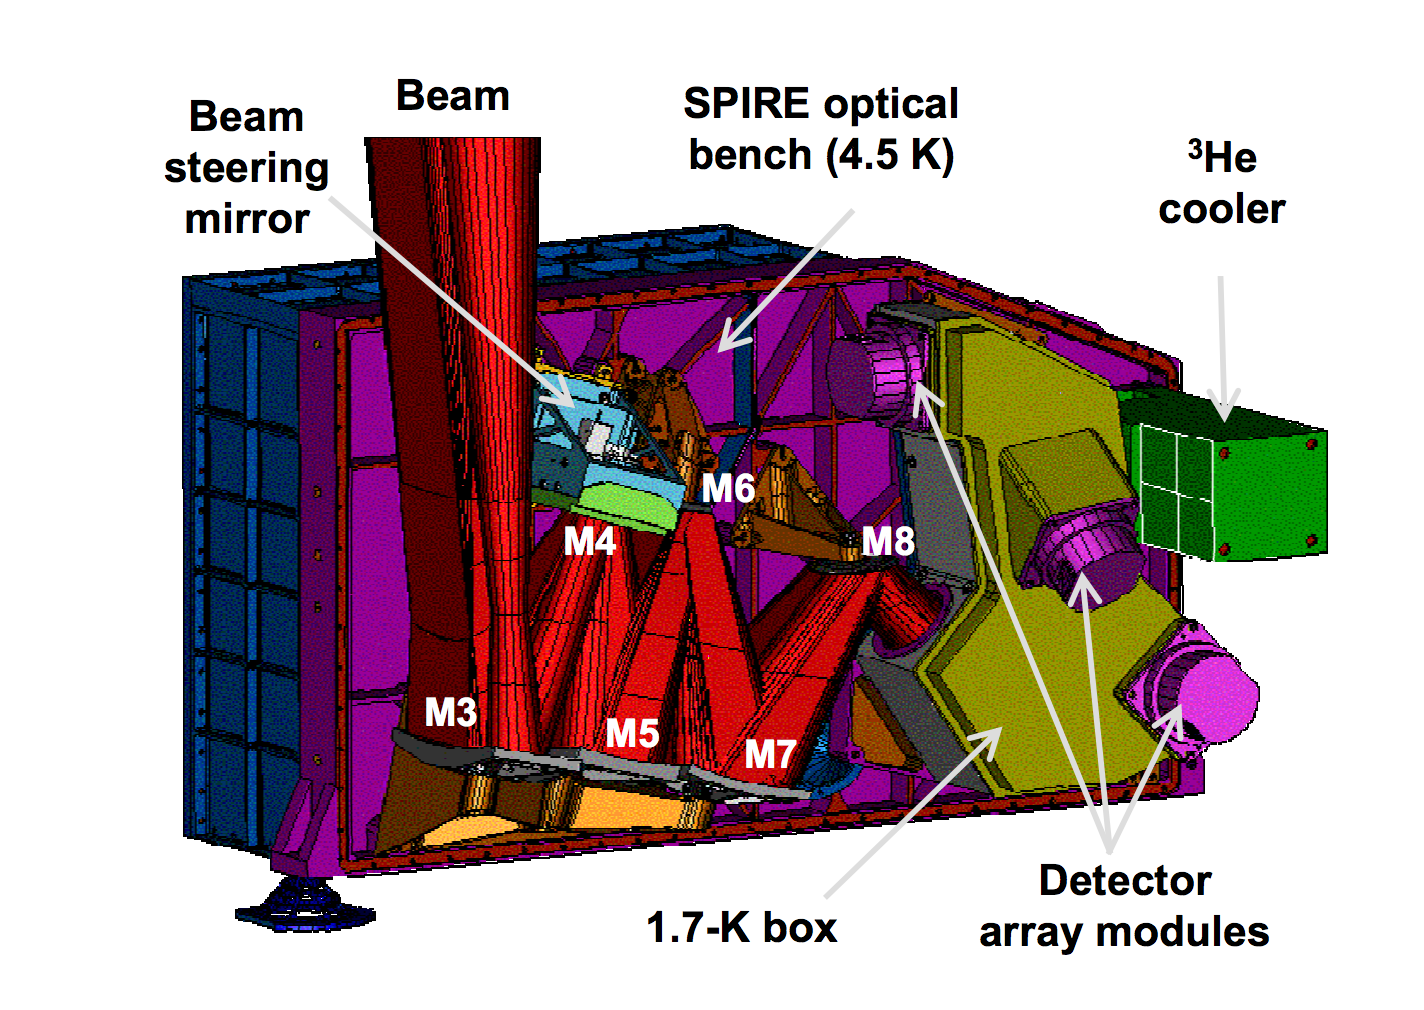
\includegraphics[width=0.8\linewidth]{figures/spire.png}
    \caption[SPIRE Photometer Layout]{SPIRE Photometer Layout \citep{griffin2010herschel}}
    \label{spire-schematic}
\end{figure}

The SPIRE instrument contains three arrays of bolometers cooled to $0.3\units{K}$. The photometer has a viewing field of 4'x8', observing simultaneously at $250\units{\mu m}$, $350\units{\mu m}$ and $500\units{\mu m}$ \citep{griffin2010herschel}. This corresponds to a diffraction limited resolution of 18'', 25'' and 36'' respectively.

Figure \ref{spire-schematic} shows the basic layout of the SPIRE optical system. SPIRE uses a series of mirrors to reflect the incoming beam onto the various instruments contained within, which are cooled by liquid $^3$He.

\begin{figure}[H]
    \centering
    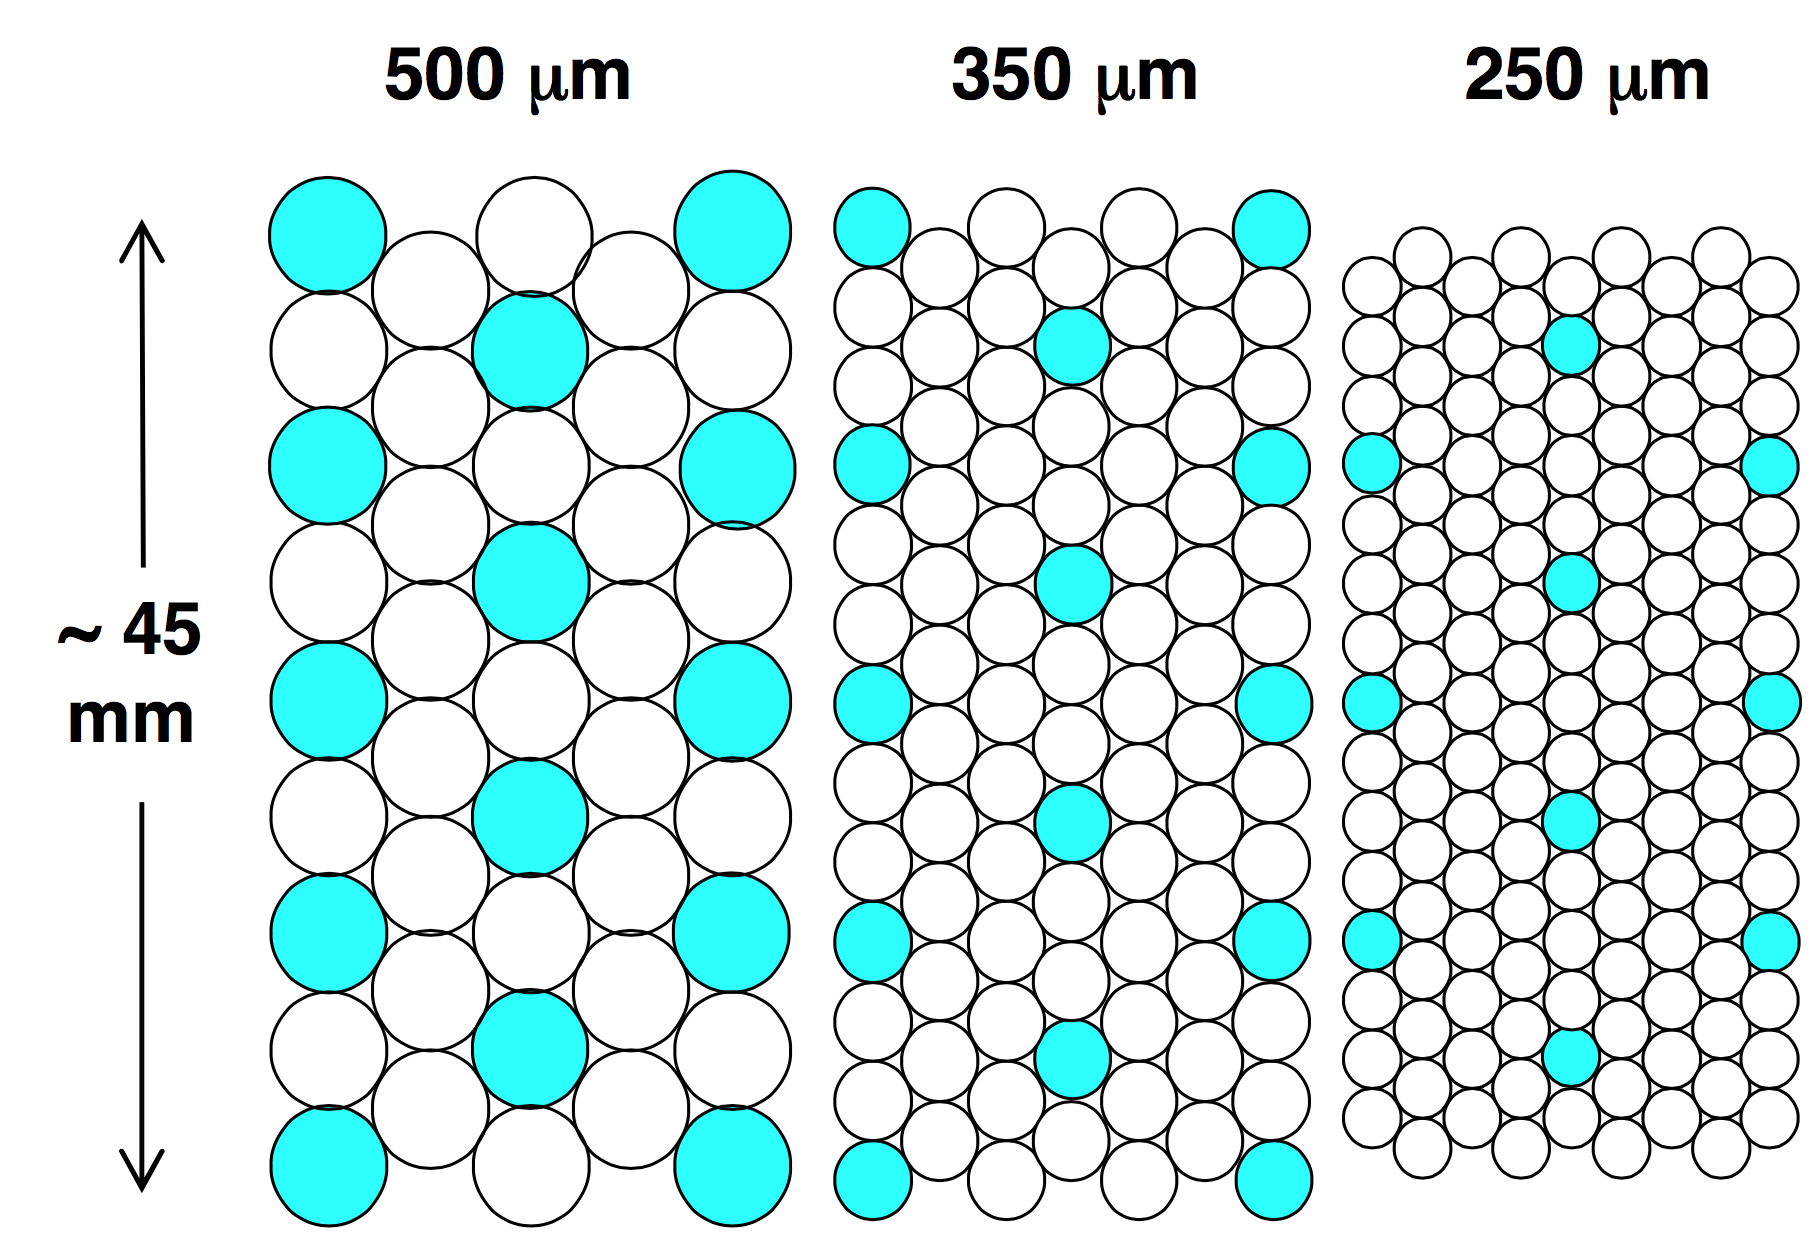
\includegraphics[width=0.8\linewidth]{figures/bolometer-layout.png}
    \caption[SPIRE Bolometer Array Layout]{SPIRE Bolometer Array Layout \citep{griffin2010herschel}}
    \label{spire-bolometer}
\end{figure}

There are three arrays of bolomerers for imaging. These arrays contain 43, 88 and 139 individual bolometers for the $500\units{\mu m}$, $350\units{\mu m}$ and $250\units{\mu m}$ band observations respectively, and are arranged as shown in Figure \ref{spire-bolometer}.

To achieve a larger field of view for observations, scans are taken across the sky, at a rate of $30''/s$ in the nominal mode, or $60''/s$ in fast mode \citep{handbook2014herschel}. The bolometer arrays are not fully filled, so the telescope scans are performed at $\pm42.4^\circ$ with respect to the Z-axis of the arrays, and the scan lines are separated by 348'' to provide overlap and good coverage. Cross scanning is performed at both the $\pm42.4^\circ$ angles providing full coverage and oversampling of the observation (Figure \ref{scan-angles}). The data for each bolometer is stored as a timeline and can later be processed into a map image.

\begin{figure}[H]
    \centering
    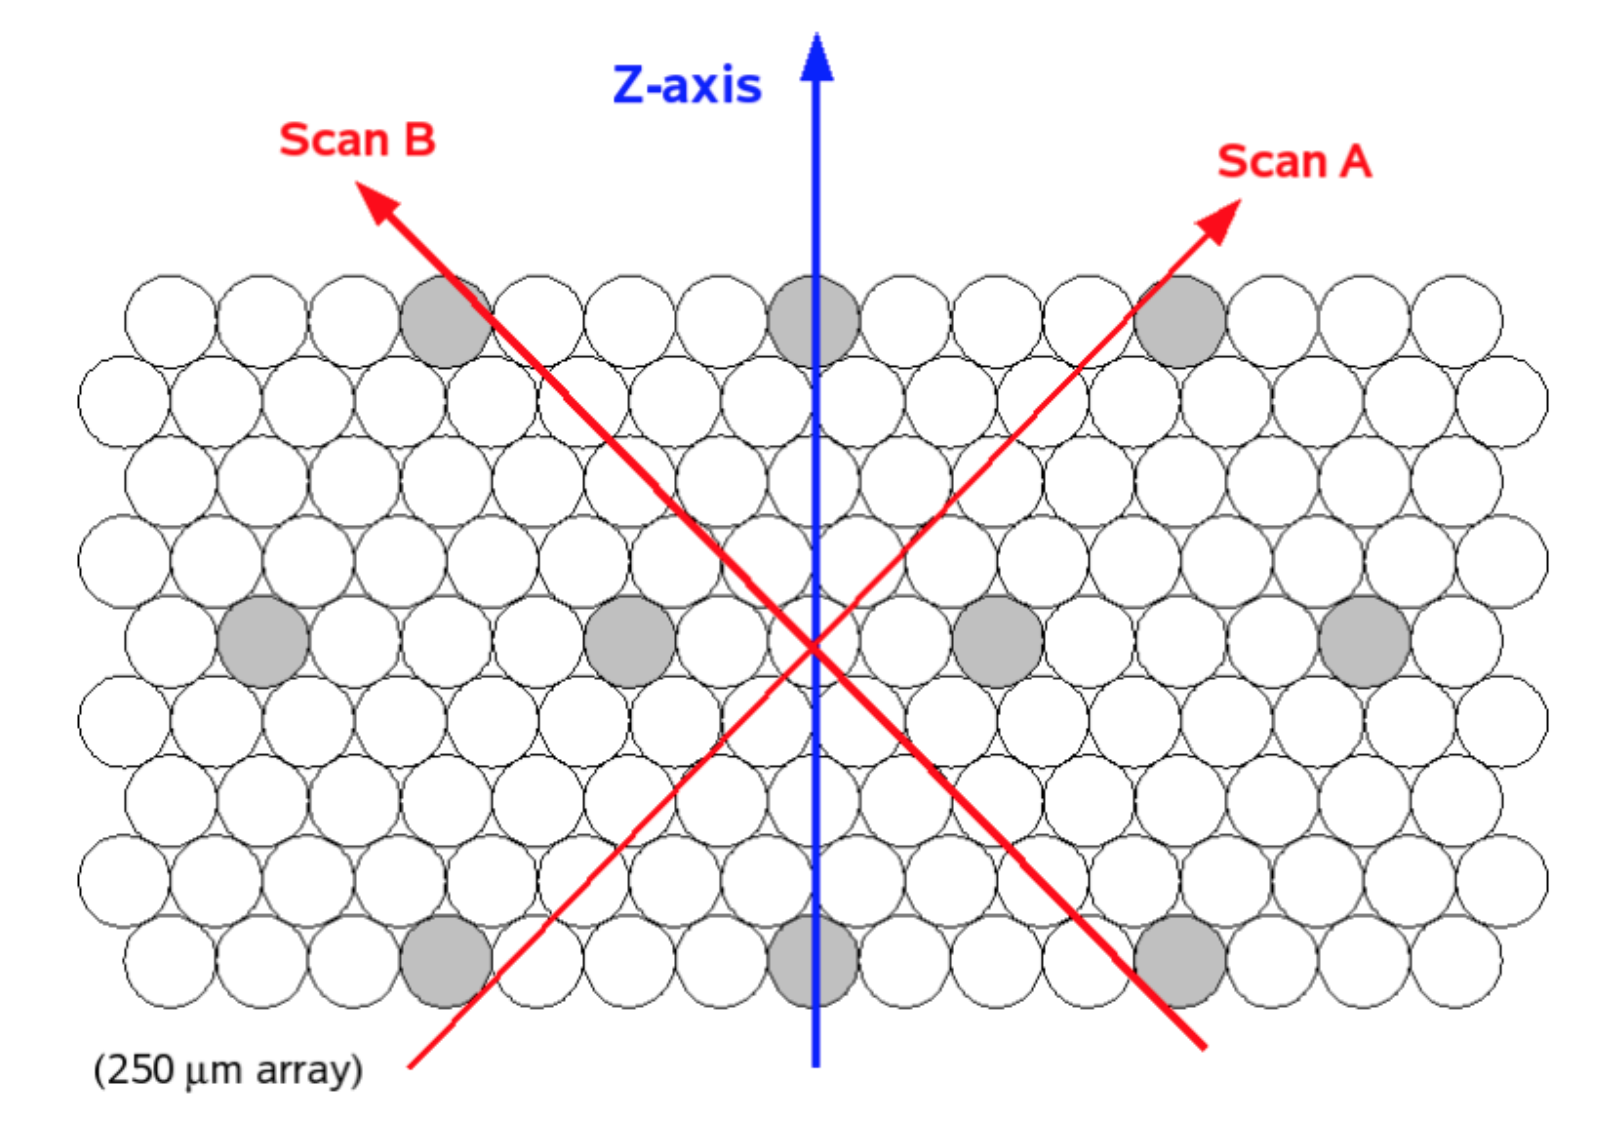
\includegraphics[width=0.8\linewidth]{figures/scan-angle.png}
    \caption[SPIRE map scan angles]{SPIRE map scan angles \citep{handbook2014herschel}}
    \label{scan-angles}
\end{figure}

The rate of sampling of this information into the timelines is greater than the limit required by Nyquist-Shannon sampling theory, and these signals are oversampled. It is this oversampling that allows for HiRes to achieve good results on the SPIRE observational data. With both PACS and SPIRE photometer data, a blackbody spectrum can be established for any observation, this is shown in Figure \ref{herschel-bb}.

\begin{figure}[H]
    \centering
    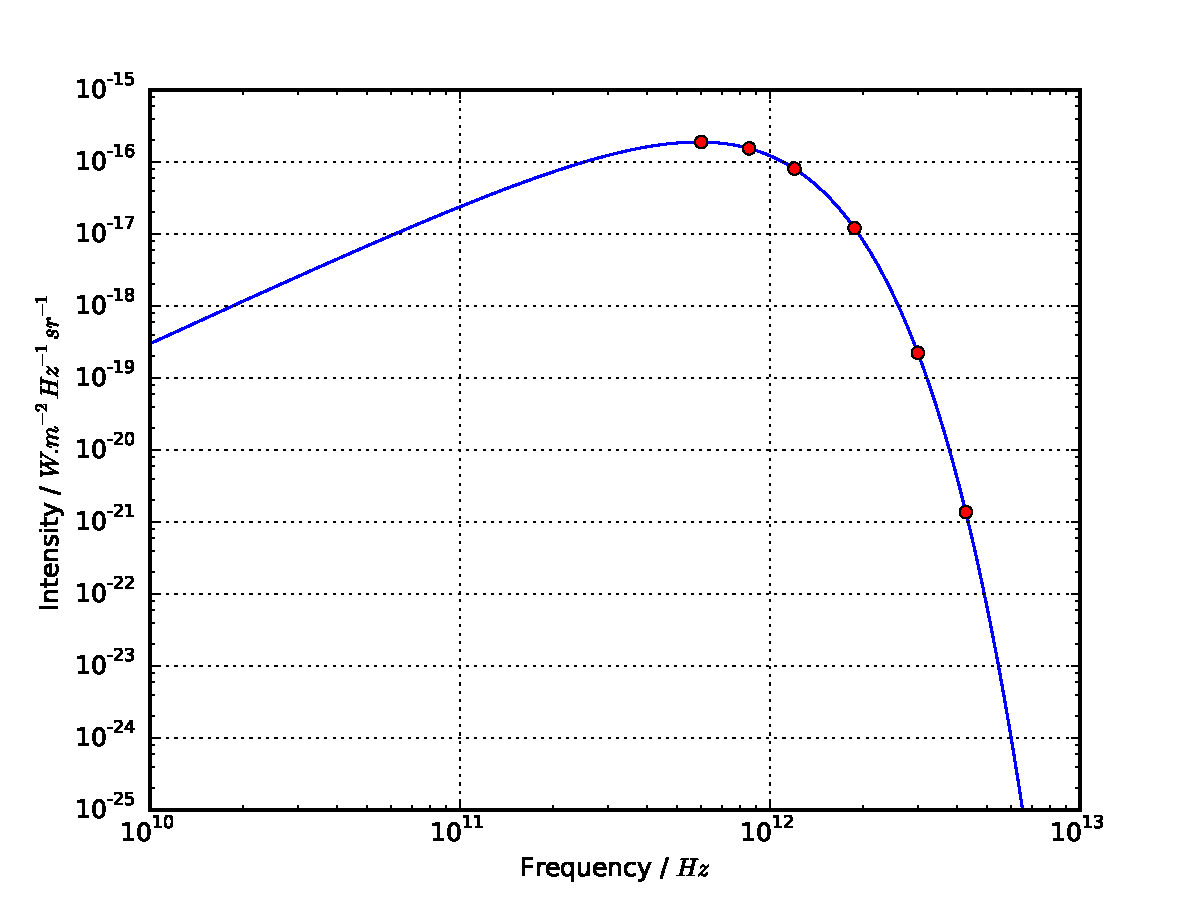
\includegraphics[width=\linewidth]{figures/bb10kHERSCHEL.pdf}
    \caption[Herschel observing frequencies for a 10K blackbody]{Herschel observing frequencies for a 10K blackbody combining both PACS and SPIRE photometers. The points show what would be the measured values for each photometer.}
    \label{herschel-bb}
\end{figure}

\subsection{Fourier Transformation}

A Fourier transform takes a source signal, and decomposes it into the various frequencies that make up that signal. In the case of a wave as a function of time, the Fourier transform will output the frequencies that make up that wave. In the case of an image the output will be the the spatial frequencies. Mathematically the Fourier of a transform is defined as in equation \ref{fft}, where $x$ is the independent variable in normal space, and $\mu$ is the transform variable in frequency space.

\begin{equation}
    f'(\mu) = \infint{ f(x) e^{-2\pi ix\mu}}{x}
    \label{fft}
\end{equation}

A Fourier transform can be reversed to give back the original function in normal space, using equation \ref{fftr}.

\begin{equation}
    f(x) = \infint{ f'  (\mu) e^{2\pi i\mu x}}{\mu}
    \label{fftr}
\end{equation}

\subsubsection{Discrete Fourier Transform}

While the Fourier transform as shown in equation \ref{fft} is useful when performing analytical analysis of some problem, it does not apply when some data set needs to be analyzed. In this case some other form is needed, and this suitable method to use is the discrete Fourier transform.

In a discrete Fourier transform, a set of samples of some function (i.e. the input data) is converted into a set of coefficients of sinusoids ordered by their respective frequencies. So for example, data sampled from a sine wave on the input function would generate a set of data with just a single value at the location of the frequency of the original sine wave.

The discrete Fourier transform is usually performed on a computer by what is known as a Fast Fourier Transform, which is usually an implementation of the Cooley-Tukey algorithm \citep{welch1967use}. Typically the fast Fourier transform routines return an image that has the same pixel dimensions as the source image, where the central pixel represents the lowest frequency component wave.

\subsection{Image Convolution}

Convolution is general method for filtering an image. A kernel is applied to each pixel of an image, and the output for each pixel is the sum of the piecewise multiplication of the kernel and the image. The kernel can be thought of as a matrix of pixel weights, and can be manipulated to produce many results, such as blurring, sharpening and edge detection on an image.

For example, an image may consist of a matrix of pixels with values:

\[
\begin{array}{|c|c|c|c|}
    \hline
0 & 0 & 0 & 0 \\
\hline
0 & 1 & 1 & 0 \\
\hline
0 & 0 & 0 & 0 \\
\hline
\end{array}
\]

And a convolution kernel of:

\[
\begin{array}{|c|c|c|}
    \hline
1 & -1 & 0 \\
\hline
1 & -1 & 0 \\
\hline
1 &  -1 & 0 \\
\hline
\end{array}
\]

By applying the kernel at each pixel location (and treating pixels beyond the edge as 0) would give the result:

\[
\begin{array}{|c|c|c|c|}
    \hline
0 & -1 & 0 & 1 \\
\hline
0 & -1 & 0 & 1 \\
\hline
0 & -1 & 0 & 1 \\
\hline
\end{array}
\]

\subsubsection{Fourier Convolution}

While performing convolution as described previously will produce a convolved image, it becomes a very time consuming operation as kernel size increases. There are also considerable difficulties with the implementation, especially with regard to convolving at the edges of an image.

There is however a solution to both of these problems. Convolution in real space corresponds directly to pointwise multiplication in the Fourier space, and deconvolution in real space to pointwise division in Fourier space \citep{katznelson2004introduction}. By performing any convolution or deconvolution in Fourier space, the time required to perform the convolution is taken almost entirely by the time performing the discrete Fourier transform. Modern data analysis libraries can perform the FFT operation incredibly fast, so when doing image convolutions with large kernels, such as a telescope beam image, Fourier convolution is usually the best choice of implementation method.

\subsection{HiRES Technique}

Originally used for data processing for the IRAS telescope launched in 1983 \citep{neugebauer1984infrared}, HiRes is a technique using the maximum correlation method to increase the fidelity of images above the nominal resolution \citep{aumann1990maximum}.

The diffraction limited resolution of the telescope can be overcome to some extent by reversing the process that limits the resolution. Essentially the image resolution is determined by a process which is essentially blurring the true sky image with the diffraction pattern produced by the telescope construction (the telescope beam). If we have a very accurate representation of this telescope beam, we can reverse this process by performing a Fourier deconvolution of the sampled image and the telescope beam \citep{lucy1974iterative}.

As HiRes is an MCM algorithm it can be applied before the image has been reconstructed from the timelines however, and operates on the data scans directly using a model of the detector response. By iterating the process it is possible to achieve significantly higher fidelity, although it is not yet clear where the limits of this technique lie with regards to SPIRE observations, nor under what conditions this method is suitable to use.


\section{Computer modeling simulated sources}
%!TEX root = spire-project.tex
\subsection{Using Spitzer Image}

Assuming a possible twofold increase in angular resolution when using HiRes, the ideal source of a truth image would be to have a telescope observing at the same wavelengths as Herschel, but with a mirror of twice the diameter. Obviously such a telescope does not exist so another source of truth images is needed, and without a physical source then we need a simulated one.

To get truth images that show information as similar as possible to Herschel observations, it was decided to use images from the Spitzer space telescope, taken at $24\units{\mu m}$ \citep{werner2004spitzer}, and filter any foreground stars if required. It was also decided early on that we could use an observation of the galaxy M74, as this had both Spitzer and Herschel observations available (Figure \ref{m74compare}).

M74 is a face-on spiral galaxy which is just under $10\units{Mpc}$ away. While M74 has a low surface brightness, it does have a large angular size of about 10'x10' making it a good source for observing spiral arm structure. As this project is concerned with the enhancement of detail rather than increasing sensitivity, M74 is an excellent source to use.

\begin{figure}[H]
    \centering
    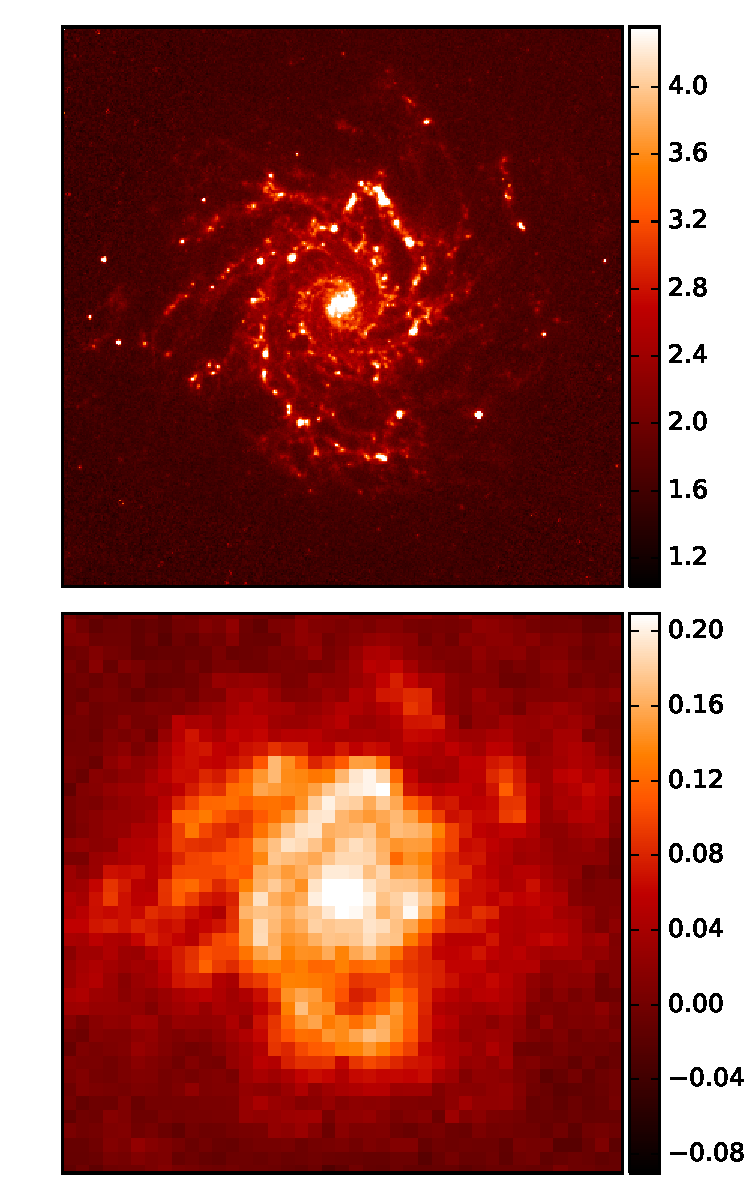
\includegraphics[width=0.9\linewidth]{figures/comparison.pdf}
    \caption[Spitzer and Herschel Observations]{Comparison of (top to bottom) Spitzer and Herschel observations of M74}
    \label{m74compare}
\end{figure}

By using the Spitzer observational data, it is then possible to create images for any telescope beam with a lower angular resolution than the original image. This can be done for instance, using the SPIRE beam, or a theoretical SPIRE beam for some imagined telescope with a larger primary mirror than Herschel. This allows the creation of both artificial observational data in the Herschel data processing pipeline, and theoretical higher resolution images for comparison.

\subsubsection{Overall Procedure}
The overall procedure for generating the simulation images is as follows:
\begin{enumerate}
    \item{Obtain the SPIRE $500\units{\mu m}$ observation data of M74}
    \item{Remove unused data products}
    \item{Obtain the Spitzer $24\units{\mu m}$ observation of M74}
    \item{Fourier convolve the Spitzer observation with the SPIRE $500\units{\mu m}$ beam}
    \item{Replace the timeline data in the SPIRE observation with the results from the Spitzer convolved image, manipulated with any noise background desired}
    \begin{enumerate}
        \item{Loop over each scan line}
        \item{Loop over each bolometer}
        \item{Loop over each data value and replace with corresponding convolved Spitzer data and noise data}
    \end{enumerate}
    \item{Build maps of simulated observation}
    \item{Build HiRes maps of the simulated data}
    \item{Create power spectra of both maps}
    \item{Create a truth image by convolving the original Spitzer data with a half-sized SPIRE beam}
\end{enumerate}

Both the nominal maps and HiRes maps can then be compared to the truth map in order to systematically study the performance of HiRes under any SNR conditions required. The method also extends as-is to the shorter wavelength observations, and observations of other objects.

\subsubsection{Creating a simulated Herschel Observation}

To generate the SPIRE observation, three primary components are needed:

\begin{enumerate}
    \item{An actual SPIRE observation to use as a data store}
    \item{An accurate SPIRE beam image}
    \item{The source Spitzer observation}
\end{enumerate}

The SPIRE observations are accessed using the HIPE software package \citep{HIPE}, and the particular observation of M74 can be found with an observation id of $1342189427$.

The beam for the long wave observations can be seen in Figure \ref{plwbeam}, and is known to very high accuracy. The Spitzer source image is shown in Figure \ref{m74compare}.

\begin{figure}[H]
    \centering
    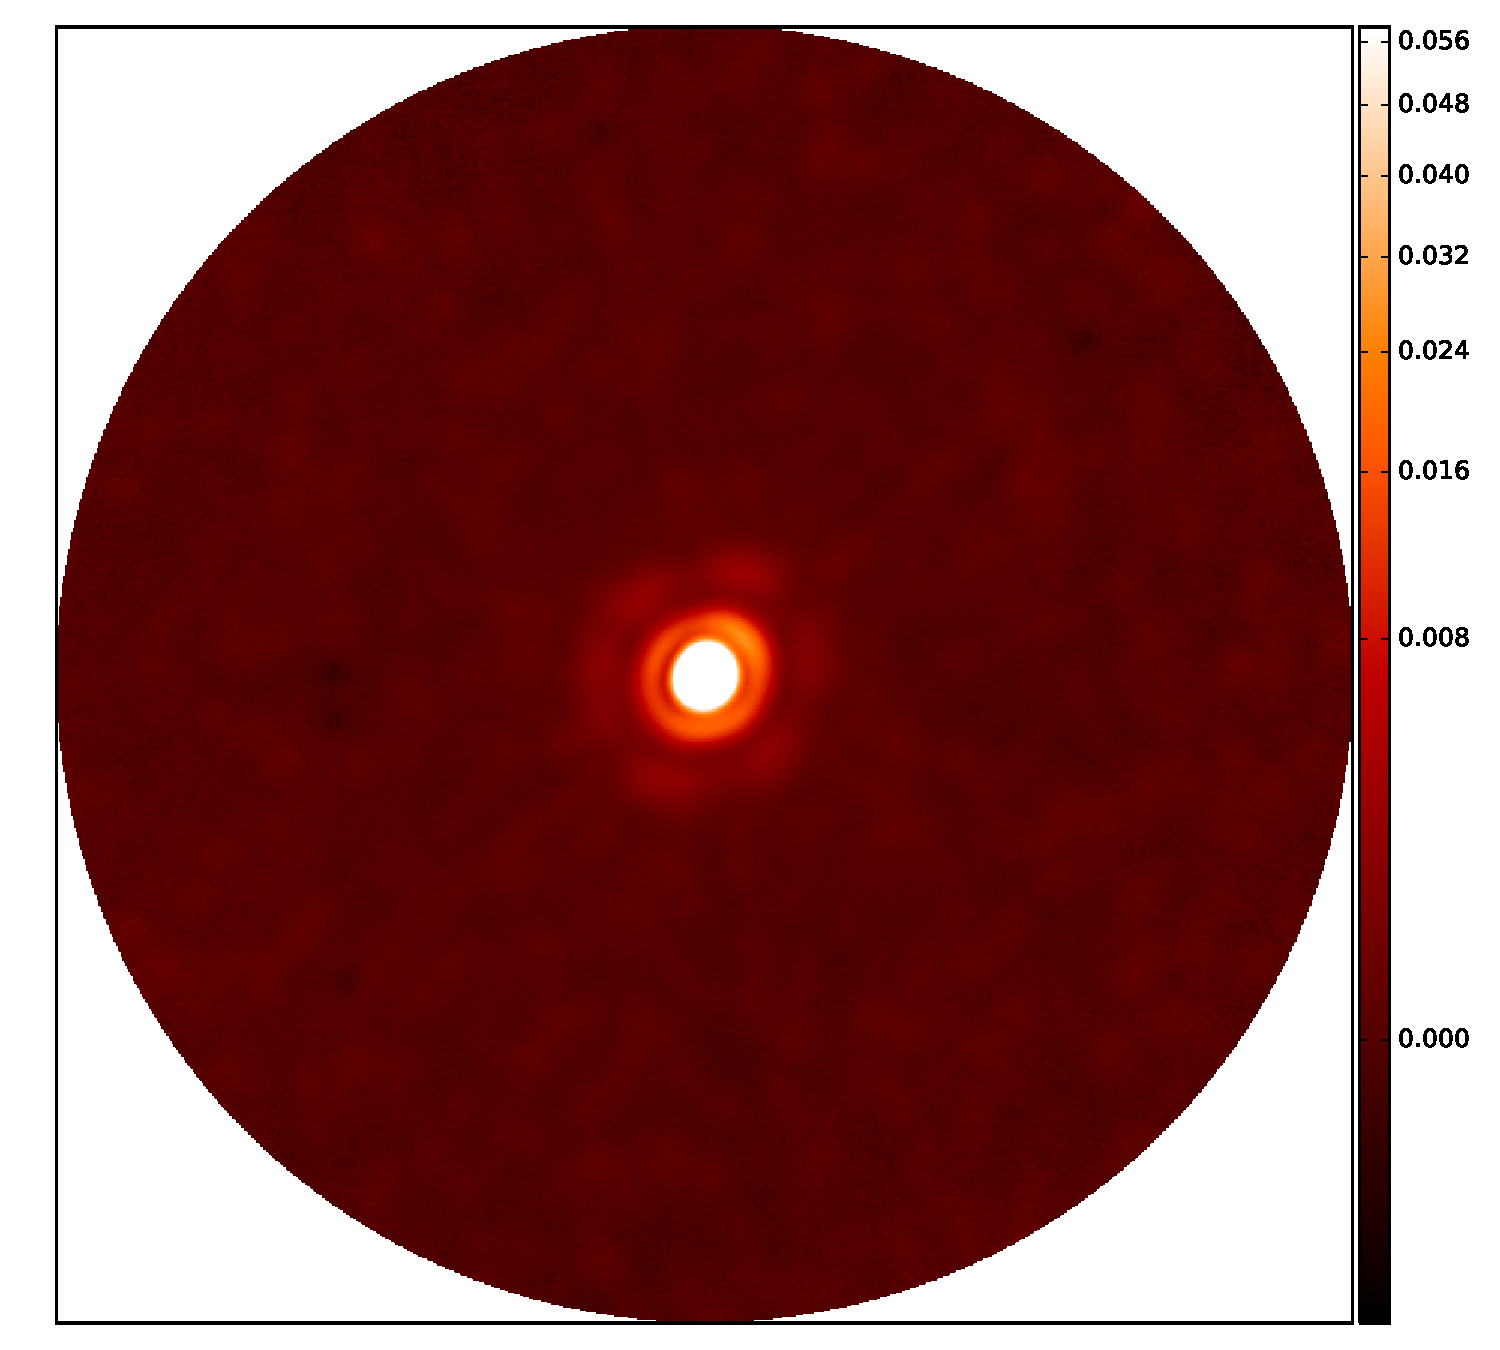
\includegraphics[width=0.8\linewidth]{figures/beam.pdf}
    \caption{SPIRE beam for $500\units{\mu m}$}
    \label{plwbeam}
\end{figure}

To create a variety of observations with varying levels of signal to noise, a dark sky observation was also chosen to provide sources of noise. While it would have been possible to artificially create random noise it was decided that using an actual source would give more realistic results. To do this we chose a wide angle observation of a 'dark' patch of sky (observation id of 1342186110) which can be sampled at various locations to generate different backgrounds for our created observation.

\subsubsection{Creating the Observations}

While I will be describing a high level overview of the process here, the actual code that generates the images can be found in the appendicies under '$spitzer.py$'.

To create any useful observational data, firstly the differences in units need to be considered. SPIRE observations, stored as a level 1 product in the HIPE software have timeline data stored in units of $\units{Jy/beam}$, and the Spitzer observations are stored in units of $\units{MJy/sr}$.

The first stage then is to convert the Spitzer data into units of $\units{Jy/pixel}$, this is done by the following operation:
\[ D = D \times 10^6 \times P \]
Where $D$ is the original image data, and $P$ is the factor necessary to convert from steradians to pixel size. In the case of these observations $P\simeq 3.8\e{-12}\units{pix/sr}$.

Next the Spitzer observation needs to be convolved with the SPIRE beam. First, the beam needs to be adjusted to have the same pixel resolution as the Spitzer image. This is done by creating a new WCS (world coordinate system) object and modifying it so that beam pixel grid resolution matches the source Spitzer image. HIPE has a tool called 'regrid' that performs this operation.

Secondly as the original beam image and Spitzer image contain NaN (invalid or no data) values, these need to be removed. In this pipeline the NaN values are removed simply by setting them to zero as they exist only at the outer regions of the beam image, and outside the area of interest in the Spitzer image. Once this has been completed, the beam and Spitzer image are transformed into Fourier space, multiplied together and then the resulting image transformed back into normal space giving a beam convolved image that now has data values in units of $\units{Jy/beam}$. NaN values can now be restored into the output image by taking the locations of NaN values in the source Spitzer image and applying them in the convolved image.

The background can the be removed from this convolved image by subtracting a median value from each pixel. Again due to there being NaN values in the image, the data needs to passed through a NaN filter before determining the background value.

Observational data in SPIRE data products is not simply stored as 2D image until mapping is performed. The data is stored in a series of time scans for each bolometer in the instrument. However as we have this timeline information in the SPIRE observation we can perform a simulation by altering this timeline data to data from a simulated scan of the Spitzer source image.

\begin{figure*}
    \centering
    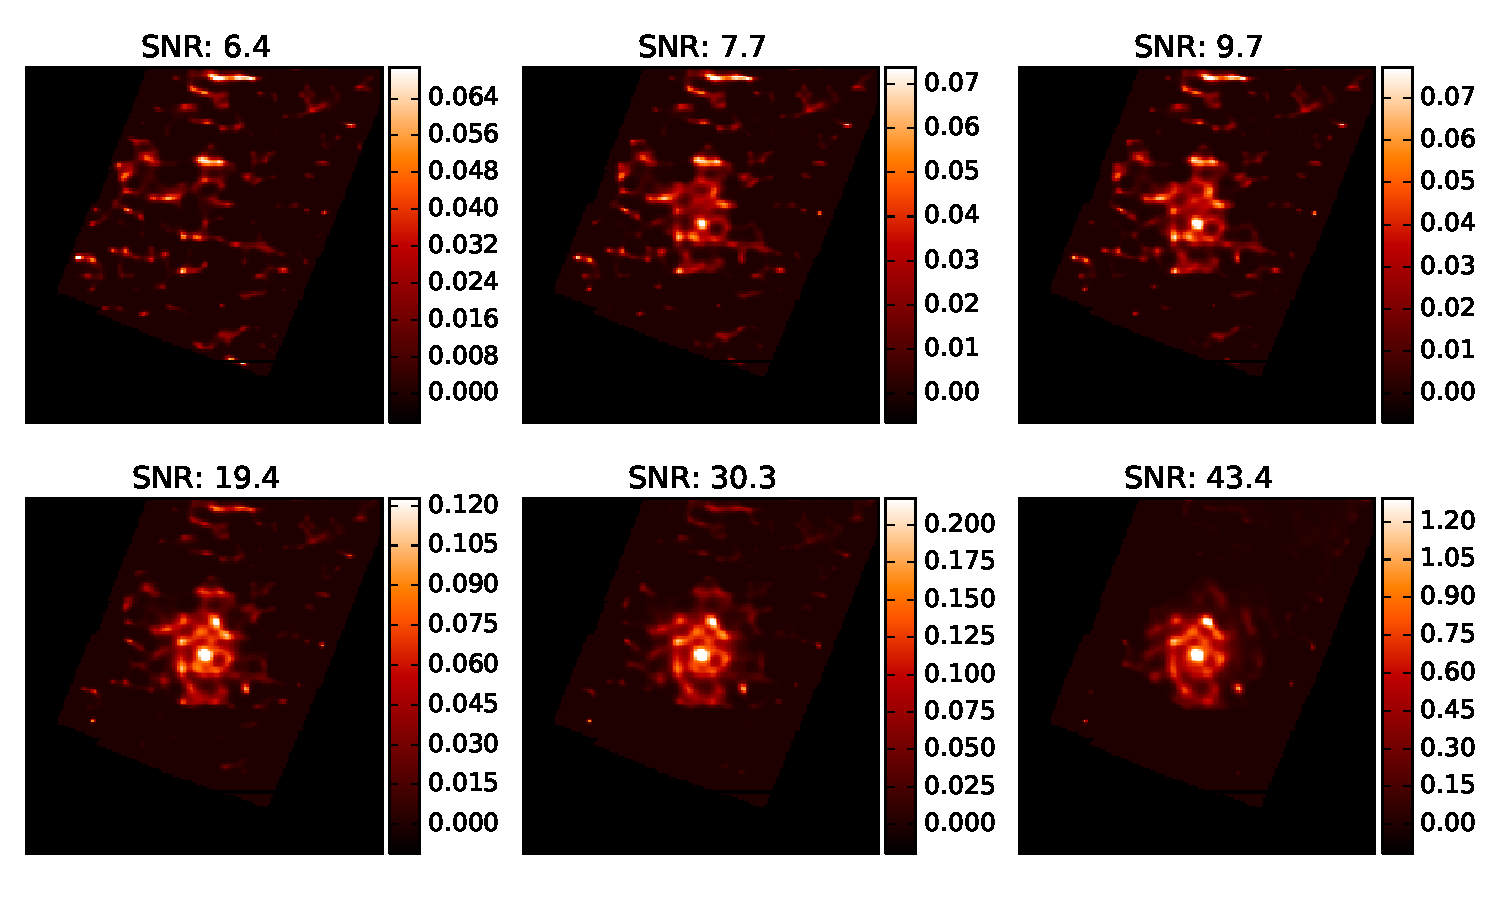
\includegraphics[width=0.9\linewidth]{figures/simulated-observations.pdf}
    \caption[Simulated observations]{Simulated observations at different signal to noise ratios, scale in Jy/beam}
    \label{simulatedobs}
\end{figure*}

To create observations with different levels of signal to noise, we also need to get the level 2 product of the chosen background source. This observation covers a much larger area than the M74 observation, so a set of locations is randomly chosen from which the background data can be obtained.

A scan line in a SPIRE observation contains data for each bolometer, and the data for each bolometer is stored as an array of signal values, with arrays for corresponding right ascension and declination values in the sky. The background value sky coordinates are obtained by taking a fixed point on the background image, with the difference from the sky coordinates of the start of the observation to the current position in the observation added to it. The Spitzer image value is obtained by simply getting the intensity at the location given by the sky coordinates in the SPIRE observation. The simulation is then performed by looping over each scan line, each bolometer and each signal value. The simulated observation intensity is then determined as
\[ D = B + I \times S \]
Where $D$ is the new observation data, $B$ is the background value, $I$ is the intensity in the Spitzer image and $S$ is the factor used to multiply the Spitzer value to give the desired signal to noise. This gives essentially an approximately fixed background noise level, to which any intensity of foreground to be added to create the images. Again NaN values need to be accounted for. Luckily these values only occur outside of the area of the observation that is being analyzed, so are again set to 0 to allow the mapping and HiRes enhancement to be performed.

Unfortunately it is not trivial to work out the SNR of the simulated image in advance, as the foreground already has it's own background noise that contributes. Instead the SNR must be determined after the image is created.

The above process is then repeated for each value of $S$ to generate a set of maps with different signal to noise ratios. Figure \ref{simulatedobs} shows how the image varies for different values of $S$.

Again, as previously mentioned this needs to be done for different background values so the effect of different features in the background can be eliminated. The whole process is repeated for different starting locations in the background images.

The end result is a set of images, both of the simulated observation and after performing HiRes, with varying signal to noise and using a variety of backgrounds. To generate this data for 9 different background locations, with 6 different signal to noise ratios each time and performing all the beam convolutions and HiRes processing takes around 6 hours on reasonably fast computer. Repeating for the higher resolution observations (medium and short wavelength) takes considerably longer, but the process is identical to that outlined above.

\subsubsection{Creating the Truth image for comparison}

To create a theoretical truth image for comparison, first the assumption is made that we can achieve around a two-fold increase in angular resolution through the use of HiRes. Again, as with the creation of the simulated Herschel observations we can use the same Spitzer image source.

Using the Herschel beam image, I create new beam that has the same properties and shape, but is half the size of the actual herschel beam, which corresponds to an identical optical system but with twice the angular resolution. To do this, I took the original beam FITS file, and altered the coordinate system so that the resulting beam has pixels with twice the angular size when mapped to sky coordinates. This is achieved by modifying the $cdelt$ property of the WCS coordinate system. This gives a beam image with the same pixel resolution, but twice the angular resolution so is in effect a beam for an equivalent telescope with twice the diameter aperture size.

Again, as with the generation of the observations, the source Spitzer image is then Fourier convolved with this new beam, giving an image that has twice the angular resolution of a Herchel observation, and should be the result of HiRes working on the simulated Herschel observations, again making the assumption that HiRes will at best give a resolution increase of a factor of two.

With this simulated truth image, there is now basis of comparison for determining how well HiRes has performed on any simulated observation, and can be compared to output images in a variety of ways.

\subsection{Storing the data for analysis}

To simplify analysis, the simulated observation, truth image and output of the HiRes routine are all saved out as FITS files. They are also coordinate aligned to show the same area of sky by matching the WCS coordinates between the three images. The data is also processd onto a new pixel grid so that each image has the same pixel resolution, chosen to match the HiRes output as this is the highest pixel resolution image created in the process. This has the advantage that pixel indices align between each image file, so comparisons can be made at a pixel level in the data, rather than having to worry about converting between sky coordinates and area coverage.

At this stage NaN values can also be restored by using the locations of NaNs in the original map before convolution, and replacing the locations in the simulated, HiRes and truth maps.

Power spectra are generated for each of the three maps, which are also saved as fits files, and the beam file returned by the HiRes routine is also saved in case this provides any useful information.

To provide a base noise image, one map is also generated containing just the noise background, without any of the Spitzer observation applied on top. The power spectra for this is also generated and saved.


\section{Quantifying HiRes improvements in image fidelity}

\subsection{SNR}
To determine the signal to noise ratios (equation \ref{SNR}) in the simulated maps, I have taken a peak signal to noise of the image, where the peak is defined as the 99th percentile of information and the noise is the root mean square pixel value of the background as defeined by an annulus outside the galaxy.
\begin{equation}
    SNR = \frac{Signal}{Noise}
    \label{SNR}
\end{equation}

\subsection{Analysing Power Spectra}
%!TEX root = spire-project.tex

\subsubsection{Calibration of spatial frequency axis}

To determine which values of spatial frequency correspond to pixel distances of the image in the Fourier space one can use a Gaussian image. A Gaussian has the advantage that the Fouier transfrom is also a Gaussian.

\begin{equation}
    f(x) \propto e^{\frac{-x^2}{2\sigma^2}}
    \label{gauss}
\end{equation}

\begin{equation}
    \mathscr{F}(f) \propto e^{-\frac{\sigma^2\omega^2}{2}}
    \label{fgauss}
\end{equation}

Disregarding amplitude, as only the width is cared about, equation \ref{gauss} shows the Gaussian function with a width paramter $\sigma$ and position $x$, and equation \ref{fgauss} shows the Fourier transform of the same gaussian in frequency space $\omega$ \citep{ozaktas2001fractional}. By fitting a guassian to the output spectra then it is possible to determine the relationship between pixel width and inverse angular distance.

\subsubsection{Determining resolution from Power Spectra}

\begin{figure*}
    \centering
    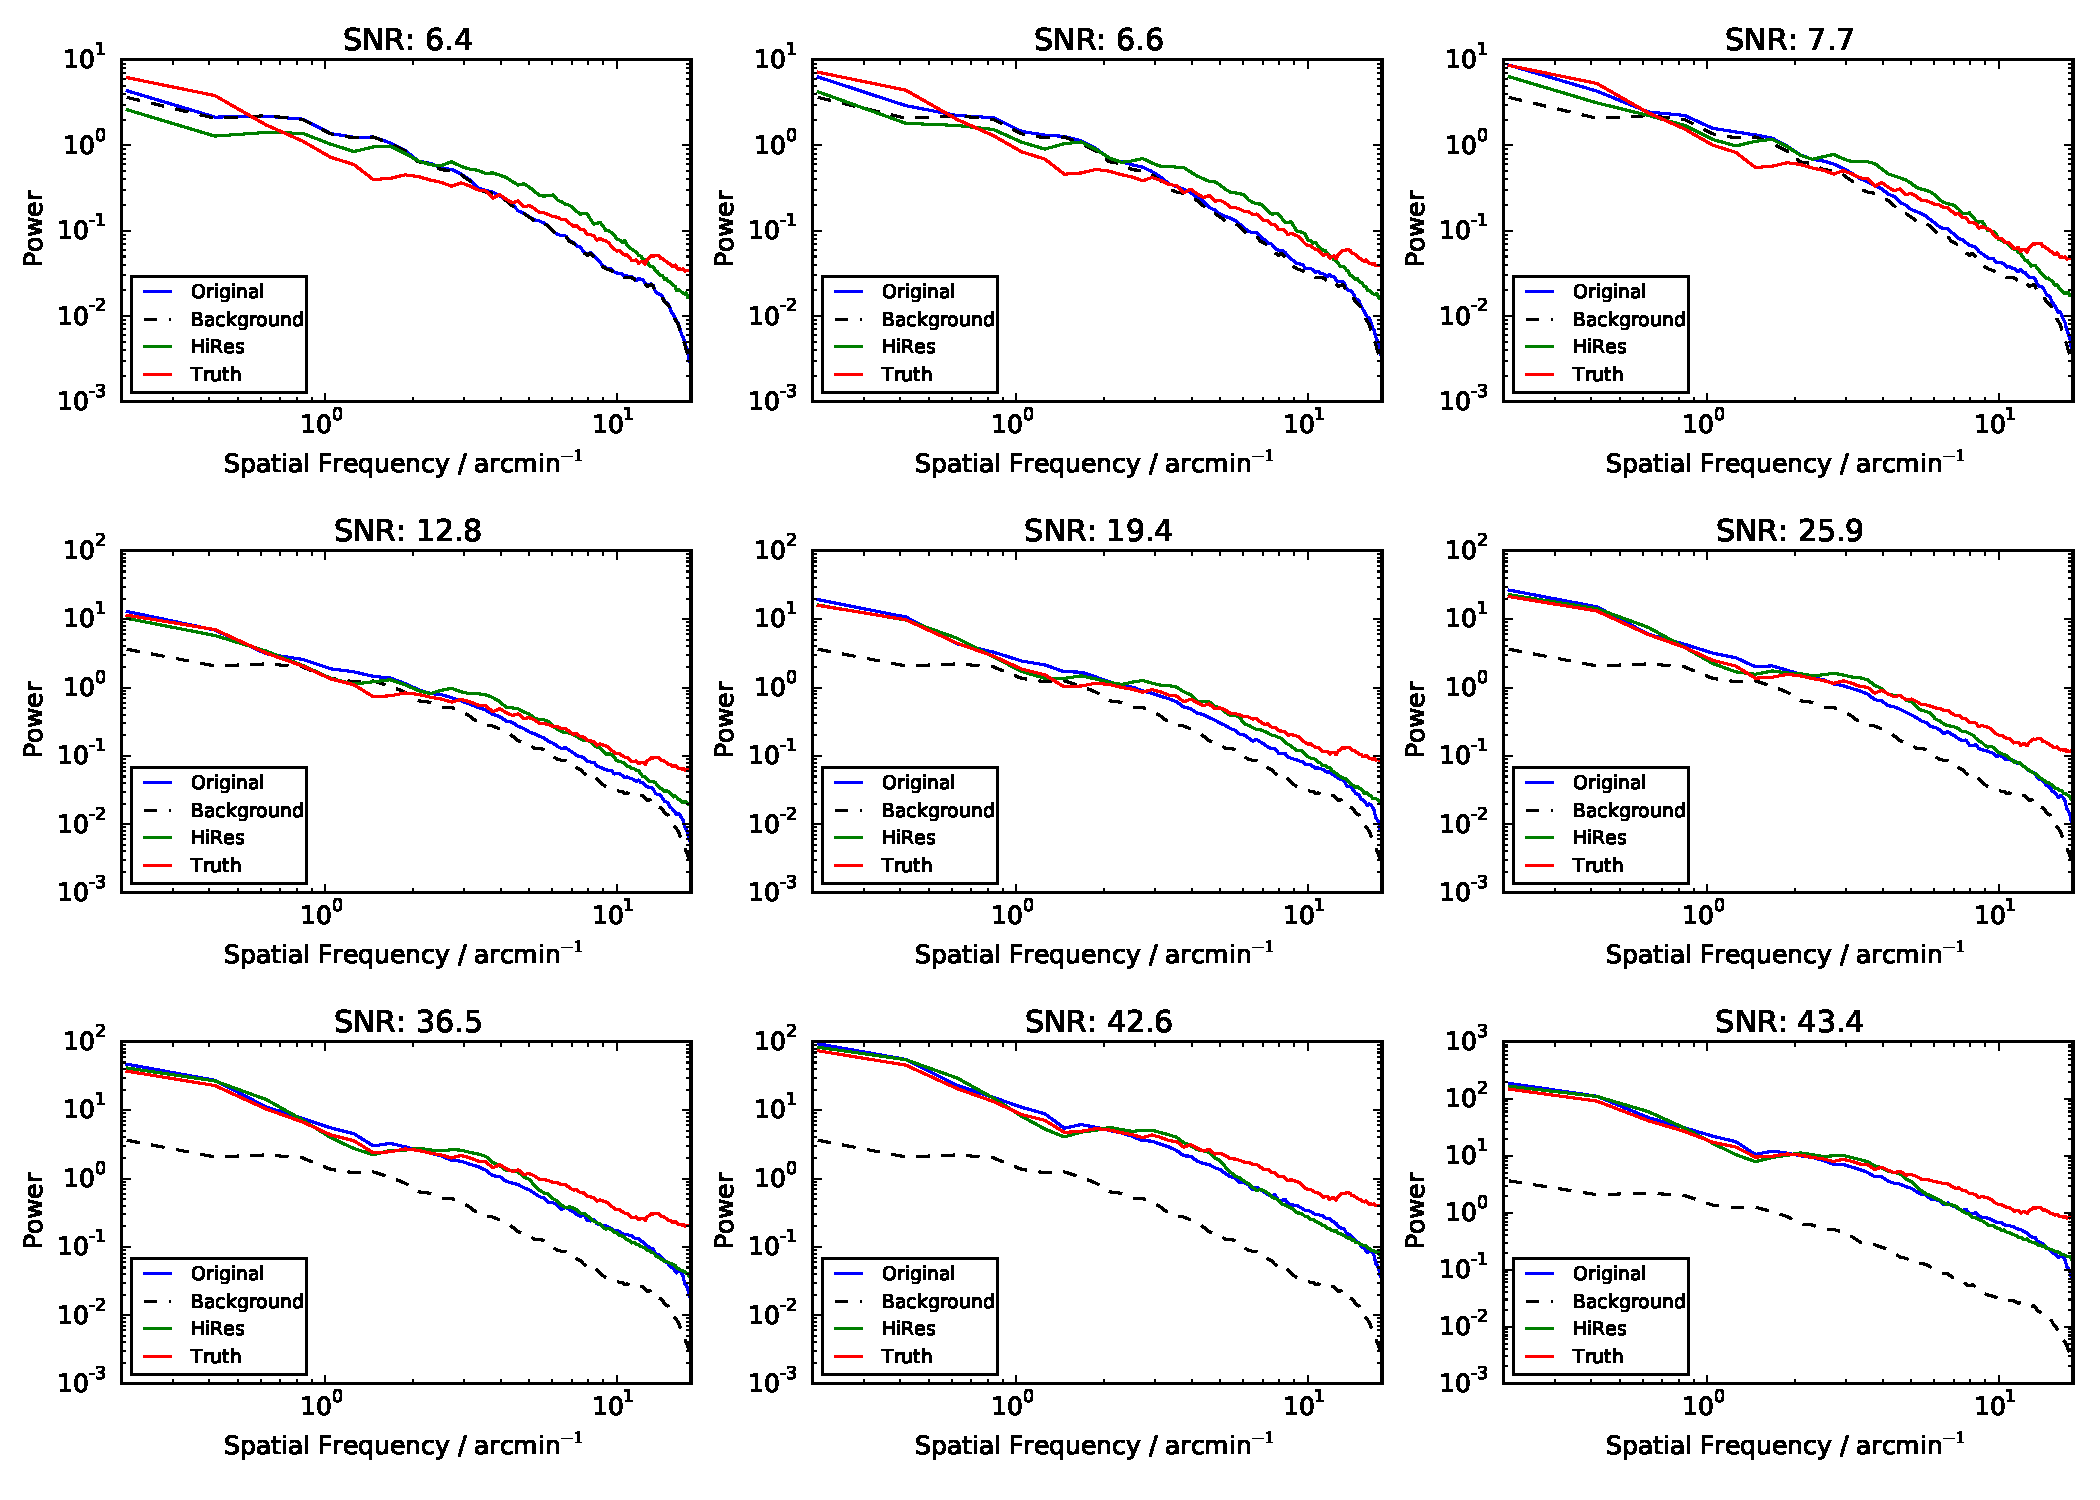
\includegraphics[width=0.9\linewidth]{figures/power-spectra.pdf}
    \caption[Power Spectra]{Power Spectra for a selection of SNR simulations}
    \label{pspectra}
\end{figure*}

When a Fourier transform of an image set is generated by the computer, a power spectrum is also produced. This roughly shows how much information there is in the waves that make up the Fourier transform.

By looking at the power spectra of the simulated image, and comparing this to the power spectra for both the HiRes output and the truth image it was hoped that information about the angular resolution improvement of HiRes could be obtained. In theory there should be a drop in the power spectrum at the point at which no more higher resolution information exists in the image.

\begin{figure}[H]
    \centering
    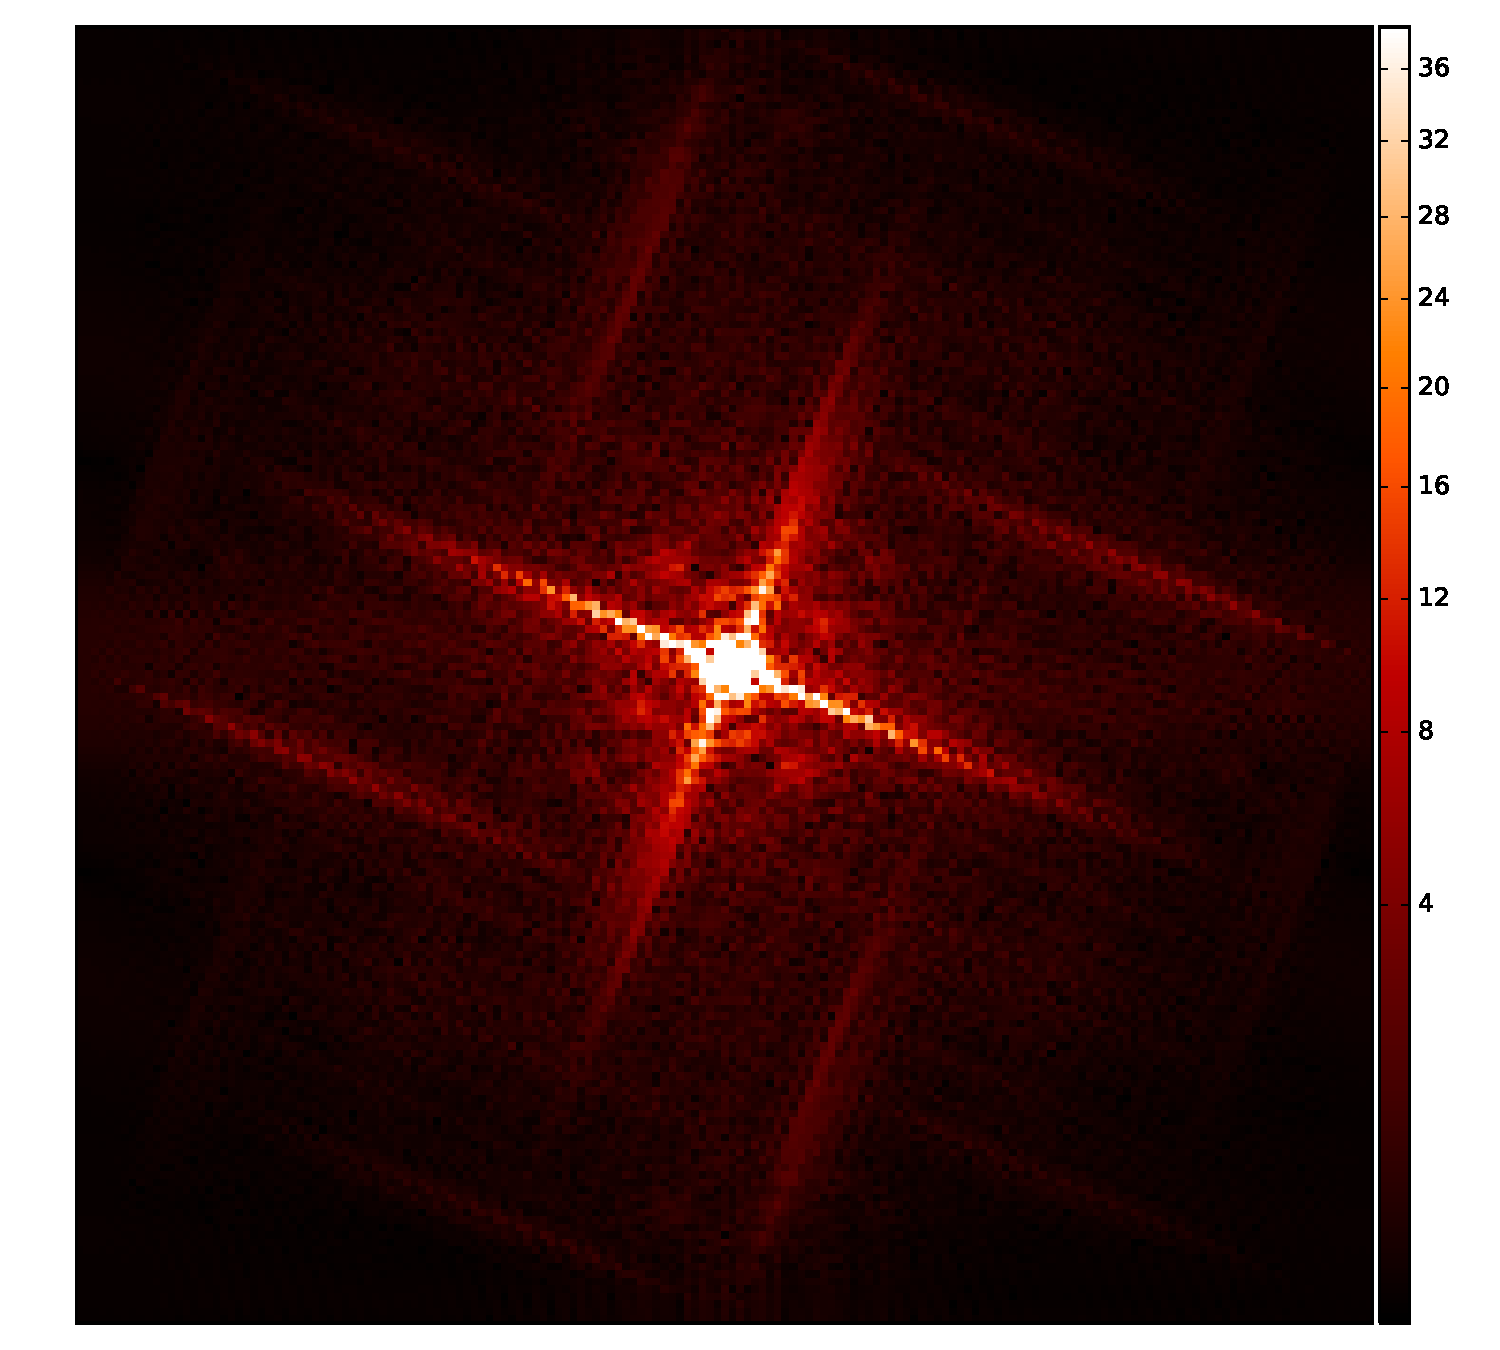
\includegraphics[width=0.8\linewidth]{figures/power-spec-sample.pdf}
    \caption[Example Power Spectrum]{Example of a generated power spectrum of an M74 observation}
    \label{spec-sample}
\end{figure}

The power spectra returned from the HIPE software routines however do not return data as typically expected. Instead of the using the central pixel as the lowest frequency wave, the returned power spectra instead is split into 4 regions, where the corner pixels of the image instead are used to indicate the lowest frequency. These spectra then need to be fixed before being used for analysis. This was done by rearranging the data such that the returned spectrum appears as expected, an example of which is shown in Figure \ref{spec-sample}. This figure is plotted with a square root normalisation as a power spectra is a square of the flux. This normalisation is shown in equation \ref{spec-scale}, where $I$ is the displayed value, $x$ is the value in the power spectrum, and $v_{min}$ and $v_{max}$ are the minimum and maximum values in the spectrum.

\begin{equation}
    I = \sqrt{\frac{x - v_{min}}{v_{max}-v_{min}}}
    \label{spec-scale}
\end{equation}

 To convert this into the graphs as seen in Figure \ref{pspectra} it is necessary to average the data at radial intervals. While this can be done by taking radial apertures and averaging the pixel values within, I decided to follow a simpler strategy that wont have any overlapping or missing pixels, or have to allow for apertures partially containing pixels. I process each of the power spectra by iterating over each pixel index, and building a histogram of the average pixel values in single pixel radial bins. This gives the 1D power spectra as shown in Figure \ref{pspectra}.

In practice however this can be very difficult to disentangle from the noise in the spectra, and I was unable to obtain any useful information from the power spectra, a sample of which is shown in figure \ref{pspectra}. It was a shame that this produced no useable information as the implementation of this part of the project took up a significant portion of the time. It is possible that further analysis of this, and performing the same analysis of different observations may allow some useful data to be obtained from this method.


\subsection{HiRes beam}

As well as generating a super-resolution map, the HiRes software routines also return a beam file. It was hopped that the returned beam may provide some indication of how HiRes has performed. To investigate this I measured the full-width half maximum of the returned beam in the hopes that this would be smaller for the higher SNR simulated observations. However this turned out not to be the case, and in fact the FWHM of the returned beam was identical for each of the source observations.

\subsection{Image Differences}
\begin{figure*}
    \centering
    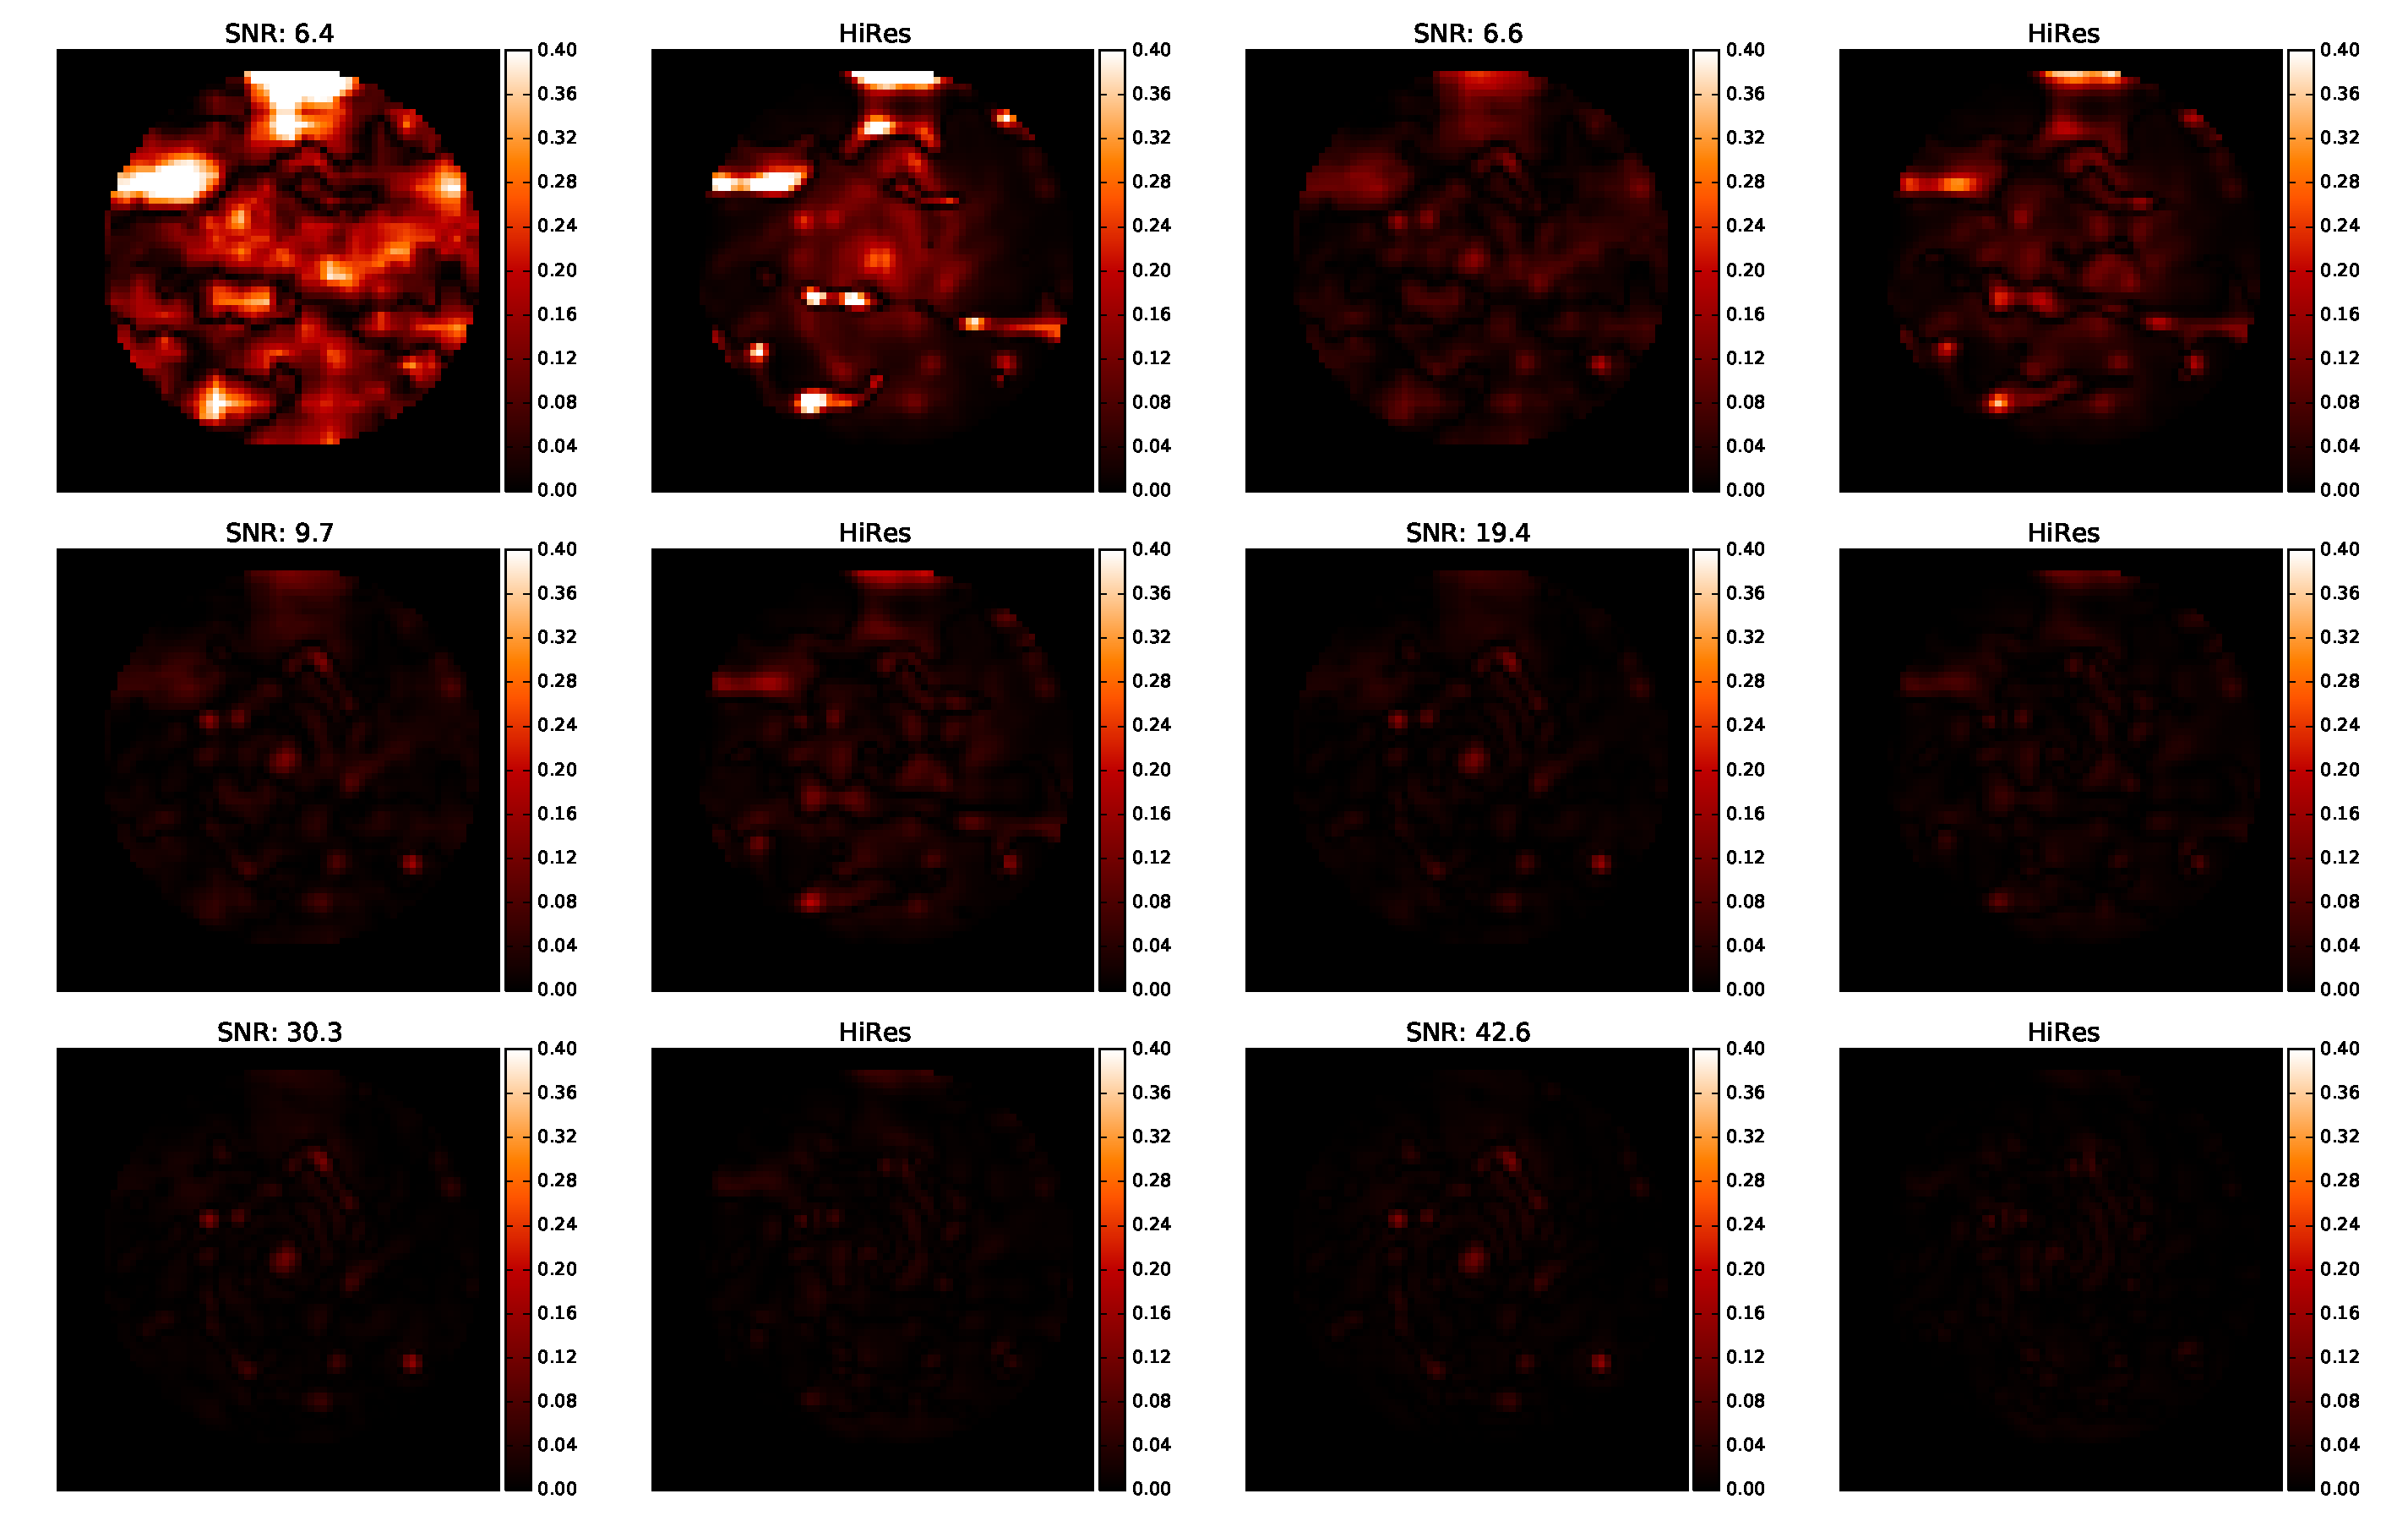
\includegraphics[width=0.85\linewidth]{figures/diff_maps.pdf}
    \caption[Difference Maps]{Difference Maps at various SNR, showing both simulated and HiRes image differences. All are shown with the same color scale, clearly demonstrating how the pixel difference decreases as SNR increases. Each pair of images is the pixel difference for the simulation and the HiRes output on that observation. All values are in Jy/beam}
    \label{diffmaps}
\end{figure*}

To clarify the terminology in this section, 'simulation' refers to the observation created from Spitzer data convolved with the SPIRE beam, 'HiRes' is the output of the HiRes routine on the simulation data, and 'truth' is the observation created from the Spitzer data convolved with the half-size SPIRE beam. When talking about any difference image, these are always taken as the data from the truth image, with either the simulation or HiRes image maps subtracted.

As we have generated a theoretical truth image it is possible to simply measure pixel differences between this truth and the output of the HiRes routines on the simulation data. By looking at the RMS (root-mean-square) pixel difference for a particular sample  it is possible to arrive at a simple number that can be used as a basis of comparison. Then, by examining the RMS pixel difference as a function of the peak signal to noise, a condition can be arrived at for when it is suitable to use HiRes on an observation.

It is not simply enough just to compare the maps as created, as in that case the RMS pixel difference would just be a function of the noise regime used in the simulation. Instead, the images need to be flux normalized and have an aperture placed over the region of interest. In the case of the M74 simulation an aperture is placed over the central galaxy, so that we are not simply comparing the noise in the background window. The total flux is then normalized between both images, and the RMS pixel difference is measured.

So the first step is to put an aperture over the image. This is done by (in the case of my data) generating a mask image that has the same dimensions as the data images. Each location in the mask is then assigned either a 0 or 1 value depending on location. Any pixel inside a radius of 30 pixels around the centre of the galaxy is assigned 1, and every pixel outside this region is assigned a value of 0. This image can then be multiplied to any other image to mask out regions outside of this zone of interest. The sum of the mask also conveniently gives the total number of pixels inside the zone of interest and can be used for instance in the calculation of averages.

Secondly the flux between the masked images needs to be normalized. In the case of two images, subscripted as 1 and 2, the data can be normalized such that they both contain the same total flux as shown in equation \ref{imnorm}.

\begin{equation}
     I_{1,x,y} = I_{1,x,y} \times \frac{\sum\limits_{x,y}{I_{2,x,y}}}{\sum\limits_{x,y}{I_{1,x,y}}}
     \label{imnorm}
\end{equation}

Once they are normalized, the simulation and original images can be subtracted from the truth image (figure \ref{diffmaps}, and the root mean square of the resulting difference maps can be calculated. Performing this analysis for the range of simulation images produced gives the result shown in figure \ref{diffresults}. As the same processing has been performed for a variety of regions in the background map, the error simply shows the standard deviation of the RMS value for each SNR sample. This also shows how the HiRes routine does reduce the flux in the background regions as the error is much less sensitive to the differences in background map itself.

\begin{figure}[H]
    \centering
    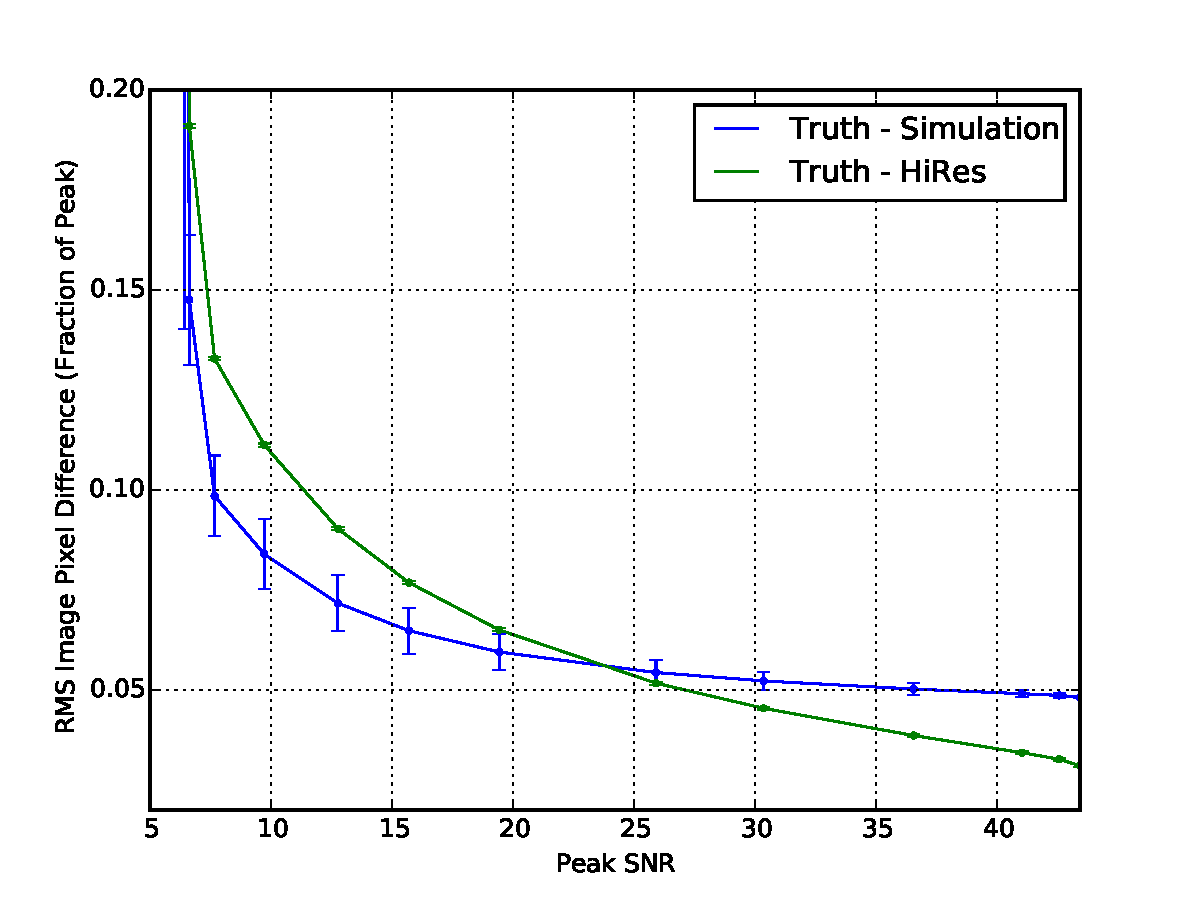
\includegraphics[width=\linewidth]{figures/differences.pdf}
    \caption[RMS Pixel differences as a function of peak SNR]{RMS Pixel differences as a function of peak SNR for the difference maps of both the simulated observations against the truth image, and the HiRes output of the simulations against the truth image. Clearly showing that for low SNR HiRes actually decreases the fidelity of the observation, but above an SNR of 30 a noticeable improvement occurs, rising rapidly as SNR further increases.}
    \label{diffresults}
\end{figure}

As shown in figure \ref{diffresults}, at low peak SNR (\textless 25) HiRes actually reduces the quality of the produced maps, as the RMS pixel difference is actually higher than when the difference is taken just for the simulation image. It is not until rising above a peak SNR of approximately 30 that the maps produced actually become better than the simulated observations themselves, and this improvement continues rapidly, rising to about a 40\% reduction in the RMS pixel difference betweek the simulated observation and the HiRes processed observation at a SNR above 40.


\section{Conclusions}

While analyzing the power spectra and beam profiles returned by HiRes didn't reveal any useful information, I did successfully develop a methodology for determining how effective HiRes has been on a simulated observation. The measuring of RMS pixel differences of both simulated and HiRes imags from a synthetic truth image proved a very successful method for obtaining whether HiRes has had a significant improvement over the unprocessed simulated observation.

I have also obtained  a value of approximately \textgreater30 for the peak SNR at which HiRes produces maps of a higher fidelity. Although this number will require refining as the analysis is expanded into shorter wavelengths and other observation types.

So in summary I have identified both a practical method, and a possible value of SNR for which HiRes would be suitable to use by default on a SPIRE observation in the Herschel data archive. There are however more questions to answer, and further study required before this can applied practically as part of the data processing pipeline.

\section{Future Work}
\subsection{Types of Observation}

This project has concentrated on an observation of a a single spiral galaxy at very low inclination. Performing the same analysis on observations of other types of galaxies and galaxies at other inclinations would give a broader picture of how HiRes works under differing circumstances.

Additionally, looking at how HiRes works on observations of inside our own galaxy. It would be expected that HiRes would behave in a different manner on more diffuse sources. A different criteria would also need to be established for how we define SNR in this case, as peak signal to noise would likely not be as useful a measurement.

All the analysis performed for this project has been done only at the long wavelength band of the SPIRE observations ($500 \units{\mu m}$). It would also be required to perform the same tests at the other wavelengths SPIRE observes, although the methods would be identical, and the implementation for this project has taken this into account so that the pipeline will work at all wavelengths.

\subsection{Beyond Doubling}

The primary assumption throughout this project has been that HiRes will provide improvements of a factor of two to the angular resolution. While this has shown to be accurate at lower signal to noise regimes, it would seem likely that this would improve as the SNR increases. Performing more analysis at this higher SNR regime would be useful. This could be done in two ways, firstly with the data already generated, the same analysis could be performed at a smaller aperture around the peak signal. Secondly observations with an innate higher SNR could also be analyzed.

As shown in the pixel difference analysis, the RMS pixel differnce approahces a stable value as SNR increase, when compared to the double resolution beam. At higher SNR this would be expected to diverge again as the resolution improvement actually increases above the factor of two.

Where I have doubled the resolution of the beam for the generation of truth images, to perform this analysis I would need to generate truth images based on smaller beams.

\subsection{SNR}

While the results I have presented give a SNR regime where HiRes is suitable, how those SNR values are determined is important for automating this in the creation of data products in the Herschel science archive. It may be that peak SNR can be automated and used for extra galactic observations such as M74 as used in this project, however for other types of observations, especially more diffuse objects this may not make sense. It may be that extra criteria are needed, such as how much of an observation likes within some SNR values, or looking further at other criteria such as properties of the power spectra not analyzed in this project.

\subsection{Proposed Continuation}

I will be continuing this project as a summer intern in the department, in order to arrive at a complete set of criteria and procedures so that the SPIRE Post-Operations Team can determine when HiRes is suitable for use throughout the data archive obtained by the Herschel Space Observatory. The plan for this would be as follows:
\begin{enumerate}
    \item{Generate test data for a larger set of observations and each wavelength}
    \item{Perform the difference analysis as described here}
    \item{Attempt to determine resolution increase limits at higher SNR}
    \item{Determine a method for determining SNR automatically on any observation}
\end{enumerate}

While it may again prove impossible to obtain a useful indicator of image resolution from the power spectra, it has been shown in this project that image differences can be used effectively so it seems likely this will be the primary method used for determining image fidelity, and this would be possible in the short window of time before September 2015.

HiRes is an iterative technique, and one area that has not been explored in this project is changing the default number of iterations used for an observation. While I found a degradation in fidelity of low SNR sources run through HiRes, it may be that with a reduced number of iterations a small improvement can be achieved. On very high SNR sources it also stands to reason that increasing the number of iterations my improve the output maps. If time allows, this may be an area that can also be explored during the internship, otherwise sticking to the default number of twenty iterations will have to be assumed correct.


\section{Acknowledgments}

As well as using the HIPE tools \citep{HIPE} much of the useful Astropy library \citep{robitaille2013astropy} was used to simplify the programming. The matplotlib library \citep{Hunter:2007} was used for figure generation, and the numpy and scipy libraries \citep{van2011numpy} were used for data analysis and processing.

\end{multicols}

\bibliography{references}

\break
\appendix
\addcontentsline{toc}{section}{Appendices}

\definecolor{mygreen}{rgb}{0,0.6,0}
\definecolor{mygray}{rgb}{0.5,0.5,0.5}
\definecolor{mymauve}{rgb}{0.58,0,0.82}

\lstset{ %
  backgroundcolor=\color{white},   % choose the background color
  basicstyle=\scriptsize\ttfamily,        % size of fonts used for the code
  breaklines=true,                 % automatic line breaking only at whitespace
  captionpos=b,                    % sets the caption-position to bottom
  commentstyle=\color{mygreen},    % comment style
  escapeinside={\%*}{*)},          % if you want to add LaTeX within your code
  keywordstyle=\color{blue},       % keyword style
  stringstyle=\color{mymauve},     % string literal style
  basicstyle=\small,
}

\providecommand{\pycodesection}[3]{
\subsection{#1}
\pycode{#2}{#3}
}

\providecommand{\pycode}[2]{
  \lstinputlisting[title=#2, breaklines=true, numbers=left, tabsize=4,language=Python]{#1}
}

\providecommand{\configfile}[1]{
  \lstinputlisting[breaklines=true, numbers=left, tabsize=4]{#1}
}

\section{Code Listings}
\pycodesection{Shared Routines}{code/common.py}{common.py}
\pycodesection{Generation of Truth Images}{code/spitzer.py}{spitzer.py}
\pycodesection{Analysis of Spectra}{code/spectra_resolution.py}{spectra\_resolution.py}
\pycodesection{Spectra unit calibration}{code/make_gauss.py}{make\_gauss.py}
\pycode{code/fft_calibration.py}{fft\_calibration.py}
\pycode{code/fft_calibration_run.py}{fft\_calibration\_run.py}
\pycodesection{Image differences}{code/differences.py}{differences.py}
\pycodesection{M74 Figures}{code/plot_m74.py}{plot\_m74.py}
\pycodesection{Beam Analysis}{code/beam_analysis.py}{beam\_analysis.py}
\pycodesection{Black Body Plots}{bbfig.py}{bbfig.py}
\break
\pycodesection{Other Figures}{code/other_plots.py}{other\_plots.py}


\end{document}
